\chapter{PHỤ LỤC}

\section{RKT Query} \label{sec:RTKQ}

\subsection{Giới thiệu}

\tab Phần giới thiệu thư viện RTK Query được trình bày theo trình tự:

\begin{itemize}
      \item Giới thiệu sơ lược thông tin của thư viện React và Redux.
      \item Từ phần trên, liên kết và trình bày quá trình hình thành và sơ lược thông tin về thư viện Redux Tookit.
      \item Từ phần trên, liên kết và trình bày sự hình thành và giới thiệu thư viện RTK Query.
\end{itemize}

\myparagraph{React và Redux}
\tab \tab Thư viện React, là một thư viện JavaScript giúp xây dựng giao diện người dùng, dùng để phát triển ứng dụng web.
Khi sử dụng React thì việc quản lý trạng thái ứng dụng (state) là một trong những vấn đề tiên quyết cần giải quyết.

Trong hệ sinh thái của React, Redux là một trong những công cụ dành cho vấn đề này.
Redux là một thư viện JavaScript, dùng để quản lý state ứng dụng, được sử dụng rộng rãi trong hệ sinh thái React.
Như hình \textit{\ref{fig:BieuDoLuotTai} \nameref{fig:BieuDoLuotTai}}, được lấy từ trang npm trends \footnote{https://npmtrends.com/, trang so sánh lượt tải của gói npm theo thời gian.}.
Ta có thể thấy được sự phổ biến của Redux đối với React qua số lượt tải của Redux, trong vòng 2 năm từ 7/2021 đến 7/2023, luôn đạt 50\% số lượt tải của React, và dao động của hai đường đo tương thích với nhau.

\begin{figure}[H]
      \centering
      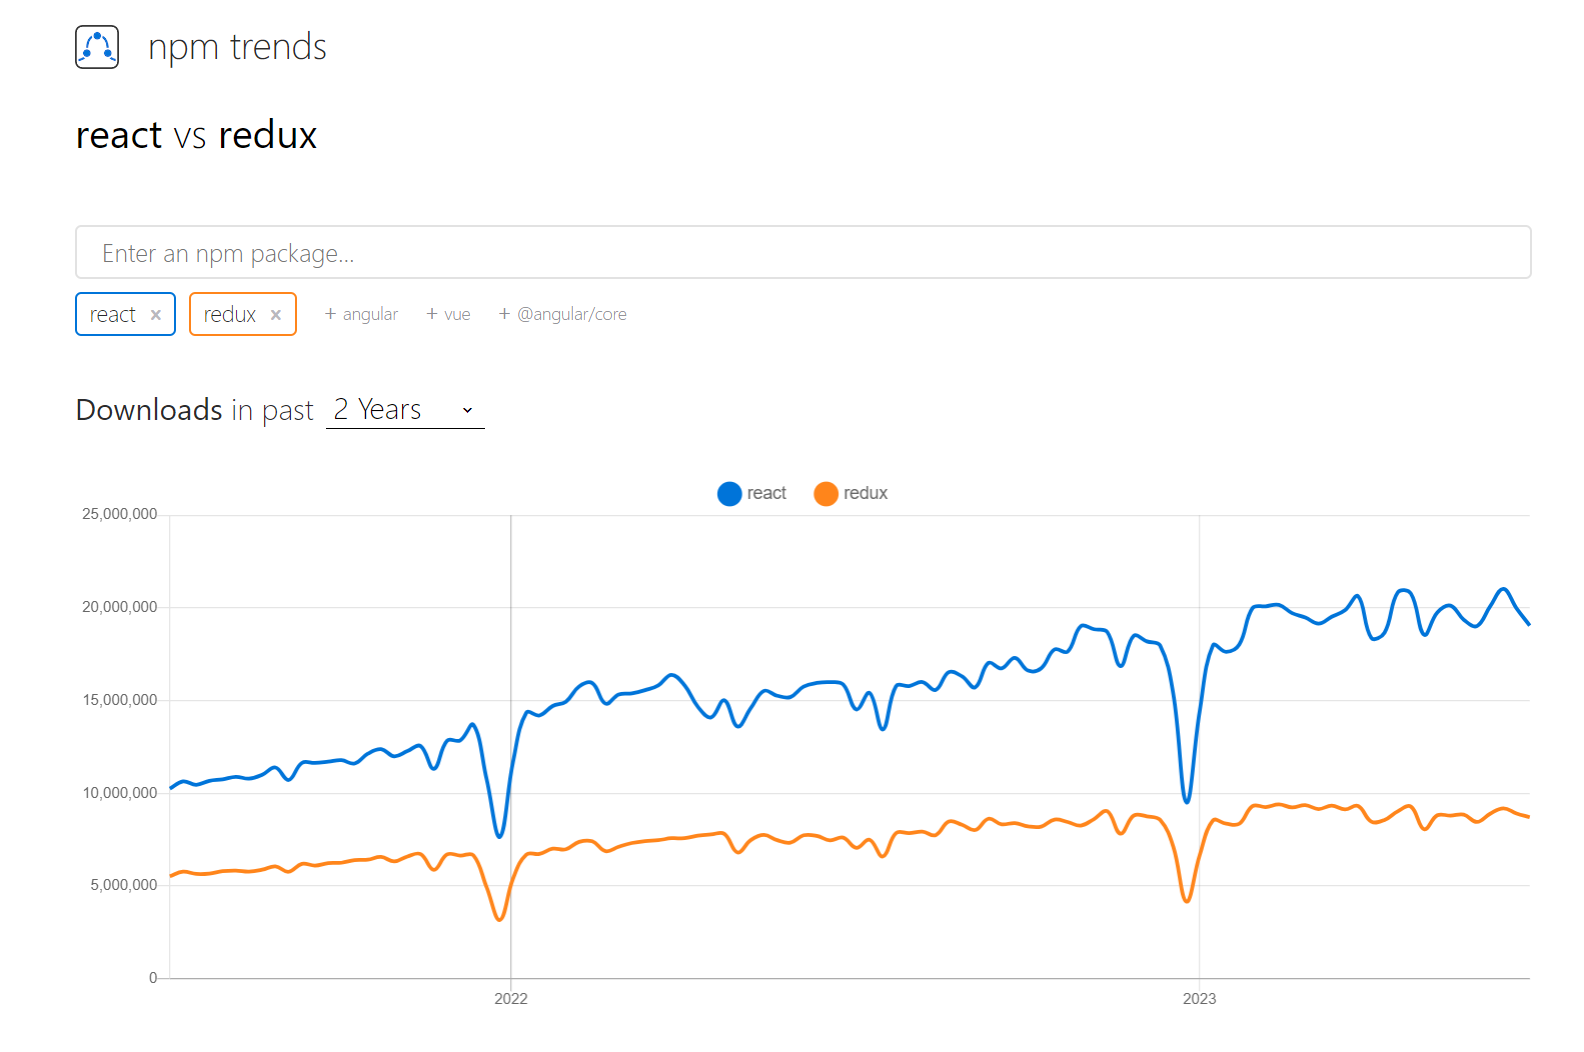
\includegraphics[width=\textwidth]{applied-thesis-chapters/chapter-6/Biểu đồ số lượt tải gói “react” và “redux” theo npm trends trong 2 năm.png}
      \caption{Biểu đồ số lượt tải gói “react” và “redux” theo npm trends từ 7/2021 đến 7/2023}
      \label{fig:BieuDoLuotTai}
\end{figure}

Vì vậy, thư viện Redux thường được chọn để giải quyết vấn đề này cho ứng dụng web được xây dựng với thư viện React.

\myparagraph{Redux Toolkit}
\tab \tab Trong quá khứ, trước phiên bản React 16.8, để có thể theo dõi trạng thái và vòng đời của một thành phần React (React component) thì sử dụng thành phần lớp React (React class component) là cách duy nhất.
Khi đó, việc sử dụng Redux trong ứng dụng React có đôi chút khó khăn và dài dòng do cú pháp, cấu trúc phức tạp.

Từ phiên bản React 16.8, với sự xuất hiện của thành phần hàm React (React functional component) là cách khởi tạo React component mới, cùng với sự xuất hiện của React Hook là cách quản lý trạng thái và vòng đời của component trong React functional component, thì Redux cũng được cải tiến bởi chính nhóm phát triển để phù hợp với sự thay đổi này.
Dẫn đến sự xuất hiện của thư viện Redux Tookit.

\textit{"Redux Toolkit là phương pháp tiêu chuẩn chính thức để viết logic Redux.
      Nó bao bọc xung quanh lõi của Redux, và chứa các gói và hàm được cho là cần thiết để xây dựng một ứng dụng Redux.
      Redux Toolkit tích hợp các thực hành tốt nhất (best practices) được đề xuất, đơn giản hóa hầu hết các tác vụ Redux, ngăn ngừa những sai lầm phổ biến và làm cho việc viết ứng dụng Redux dễ dàng hơn."} \cite{chap4bib1}
\par

\myparagraph{RTK Query}
\tab \tab Khi xây dựng ứng dụng web thì việc tương tác và quản lý dữ liệu API cũng là một vấn đề tiên quyết.
Khi phát triển ứng dụng có sử dụng Redux, nếu muốn đưa dữ liệu nhận được từ API lên trạng thái toàn ứng dụng (global state) thì ta thực hiện chuyển dữ liệu này lên Redux store (đối tượng quản lý global state của Redux).
Redux là một thư viện đồng bộ nhưng tác vụ tương tác với API lại là tác vụ bất đồng bộ, nên thực hiện việc này sẽ có khó khăn là mã dài dòng và khó quản lý lỗi.

Để giải quyết vấn đề này, Redux Tookit có cung cấp hàm createAsyncThunk giúp đơn giản hóa quá trình tạo ra tác vụ bất đồng bộ.
Tuy nhiên, người dùng vẫn phải viết một số lượng logic đáng kể để quản lý dữ liệu ghi đệm và trạng thái tải.
Cũng như khó khăn trong việc quản lý lỗi.
Redux Toolkit Query (RTK Query) là một thư viện bổ sung cho Redux Toolkit.
Cũng được phát triển bởi chính nhóm phát triển thư viện Redux.
Thư viện được phát triển với vai trò như một công cụ tương tác, quản lý dữ liệu khi tương tác với API cho ứng dụng Redux.
\par

\textit{“RTK Query là một công cụ lấy dữ liệu (fetching) và lưu đệm (caching) mạnh mẽ.
      Nó được thiết kế để đơn giản hóa các trường hợp phổ biến khi tải dữ liệu trong một ứng dụng web, loại bỏ nhu cầu viết thủ công các logic lấy dữ liệu và caching của bạn.}
\par

\textit{RTK Query là một addon tùy chọn được bao gồm trong gói Redux Toolkit, và chức năng của nó được xây dựng trên các API khác trong Redux Toolkit.“} \cite{chap4bib2}
\par

Dữ liệu và trạng thái của API được tạo với RTK Query được lưu trữ và quản lý trên store của Redux.
Thiết kế của RTK Query được lấy cảm hứng từ các công cụ phổ biến, tiên phong trong giải pháp lấy dữ liệu API như Apollo Client, React Query, Urql và SWR.
Vậy nên việc sử dụng RTK Query là giải pháp cho tương tác API kết hợp với Redux Tookit trong ứng dụng sẽ giúp cho việc quản lý trạng thái ứng dụng và truy vấn mạng trở nên đơn giản, dễ dàng và hiệu quả hơn.

\subsection{Các chức năng của RTK Query}

\tab Thư viện RTK Query hỗ trợ đa dạng chức năng cho truy vấn mạng, tương tác API.
Sau đây là mô tả một số chức năng nổi bật của thư viện RTK Query và có được sử dụng trong phạm vi khóa luận.

\myparagraph{Endpoints, Queries và Mutations}
\tab \tab Việc tương tác với API trong RTK Query xoay quanh việc cài đặt các endpoint.
Endpoint trong RTK Query được định nghĩa trong hàm createApi của thư viện.
Để định nghĩa một endpoint, chúng ta cần cung cấp các thông tin như tên endpoint (là duy nhất trong phạm vi của hàm createAPI) , địa chỉ URL của API, phương thức của endpoint (phương thức HTTP, thông tin này là tùy chọn, mặc định sẽ tùy theo loại endpoint mà ta sử dụng).
Có thể sử dụng các endpoint đã được định nghĩa trong các component của ứng dụng bằng cách sử dụng hook tương ứng.
Các hook này được sinh ra tự động bởi RTK Query và có tên được đặt dựa trên tên của endpoint.
Ví dụ, nếu endpoint được định nghĩa theo loại Query endpoint và có tên là "getUsers", thì hook để sử dụng endpoint này sẽ có tên là "useGetUsersQuery".
Ngoài ra, cũng có thể sử dụng các endpoint  qua đối tượng trả về của hàm createApi, không qua hook.
Có hai loại endpoint trong RTK Query là Query endpoint và Mutation endpoint.

\begin{itemize}
      \item \textbf{Query endpoint} khuyến cáo nên được sử dụng khi lấy, truy xuất dữ liệu từ API.
            Khi sử dụng endpoint này, theo mặc định, query endpoint sẽ tự động thực thi khi component sử dụng nó được hiển thị.
            RTK Query sẽ kiểm tra xem dữ liệu đã được lưu trong store hay chưa.
            Nếu có, dữ liệu đã có trong bộ đệm sẽ được trả về mà không cần gửi yêu cầu đến server.
            Nếu chưa có, yêu cầu sẽ được gửi đến server để lấy dữ liệu mới nhất.
      \item \textbf{Mutation endpoint} khuyến cáo nên được sử dụng khi thay đổi dữ liệu, làm cũ dữ liệu trong store qua API.
            Không như query endpoint, mutation endpoint không được thực hiện tự động mà phải gọi tới mỗi khi sử dụng.
            Endpoint này có thể sử dụng để đánh dấu dữ liệu đã cũ trong store, ra hiệu cho các endpoint có liên quan làm mới lại dữ liệu, ví dụ như component có sử dụng Query endpoint sẽ lấy dữ liệu mới, loại bỏ dữ liệu đã cũ trong store.
\end{itemize}

\myparagraph{Các lifecycle hook và Streaming Update}
\tab \tab Endpoint của RTK Query có cung cấp nhiều lifecycle hook mạnh mẽ, hỗ trợ rất nhiều trong việc đóng gói các logic đi kèm bên trong chính endpoint đó.
Các lifecycle hook tiêu biểu được cung cấp trong cả Query endpoint và Mutation endpoint là transformResponse,  transformErrorResponse, onQueryStarted và onCacheEntryAdded.
Đặc biệt, trong Query endpoint có cung cấp hook providesTags và trong Mutation endpoint có cung cấp hook invalidatesTags.
Chi tiết của các hook này như sau:

\begin{itemize}
      \item \textbf{transformResponse:} dùng để cài đặt thay đổi, biến đổi dữ liệu (data) được trả về.
            Dữ liệu được trả về phải đi qua hook này trước khi được lấy ra từ endpoint
      \item \textbf{transformErrorResponse:} tương tự như transformResponse nhưng dành cho đối tượng lỗi (error).
      \item \textbf{onQueryStarted:} đây là một hook bất đồng bộ, các cài đặt trong hook này sẽ được thực hiện trước khi request của endpoint được gửi đi. Hook này có cung cấp đối tượng LifecycleApi chứa các phương thức để tương tác với dữ liệu, tham số từ endpoint.
      \item \textbf{onCacheEntryAdded:} đây cũng là một hook bất đồng bộ, các cài đặt trong hook sẽ được thực hiện khi có một mục đệm (cache entry) được thêm vào.
            Cache entry là một bộ dữ liệu của một endpoint với tham số truyền vào query đó.
            Như đã nói, RTK Query cache dữ liệu của endpoint để tối ưu số lần request, nên nếu có hai nơi gọi đến cùng một bộ endpoint và tham số thì dữ liệu sẽ được chia sẻ cho nhau.
            Vì vậy, lần đầu tiên bộ endpoint và tham số được gọi là lần cache entry được thêm vào.
            Hook này có cũng cấp đối tượng CacheLifecycleApi có tác dụng tương tự với LifecycleApi từ onQueryStarted.
            CacheLifecycleApi còn có cung cấp thêm hai thuộc tính là cacheDataLoaded và cacheDataRemoved để hỗ trợ ta có thể cài đặt đồng bộ trong hook.
      \item \textbf{providesTags:} Hook chỉ tồn tại trong Query endpoint.
            Hook giúp cho các Query endpoint tự động làm mới dựa trên các thẻ (tag) mà ta gắn vào.
      \item \textbf{invalidatesTags:} Hook chỉ tồn tại trong Mutation endpoint.
            Hook giúp xác định cache data nào sẽ được tìm nạp lại hoặc xóa khỏi store.
            Khi Mutation endpoint có gắn tag được gọi, dữ liệu nằm trong Query endpoint có tag tương tự sẽ bị đánh dấu là đã cũ.
            Nếu Query endpoint có dữ liệu đã bị đánh dấu cũ thì endpoint đó sẽ được thực hiện gọi lại để làm mới dữ liệu.
\end{itemize}

Trong onQueryStarted và onCacheEntryAdded của Query endpoint, hai đối tượng LifecycleApi và CacheLifecycleApi đều có cung cấp thêm thuộc tính updateCachedData.
updateCachedData hoạt động như một hàm hỗ trợ việc cập nhật dữ liệu lên đối tượng data của endpoint.
updateCachedData thay đổi dữ liệu giống với cách reducer của Redux.
\par

Có thể điều chỉnh cấu hình endpoint trong cài đặt hay trên hook để thay đổi hành vi của các endpoint.
Một trong những hành vi tiêu biểu nhóm cần trong phạm vi thực hiện khóa luận là cập nhật dữ liệu liên tục (streaming update).
Ta khởi tạo kết nối socket hay event source trong hook onCachedEntryAdded, phối hợp với sử dụng cacheDataLoaded và cacheDataRemoved để thực hiện hành vi này, chi tiết như đoạn trích ở dưới.
\par

\textit{“… bạn sẽ await cacheDataLoaded để xác định thời điểm dữ liệu đầu tiên được tải xuống, sau đó sử dụng tiện ích (utility) updateCacheData để áp dụng các streaming updates khi nhận được tin nhắn (messages).
      updateCacheData là một callback do Immer cung cấp, nhận bản draft của giá trị cache hiện tại.
      Bạn có thể biến đổi giá trị draft để cập nhật giá trị đó khi cần dựa trên các giá trị nhận được.
      RTK Query sau đó sẽ gửi một hành động áp dụng một bản vá lỗi khác dựa trên những thay đổi đó."} \cite{chap4bib3}

\newpage
\section{Reactive Programming và RxJS}

\subsection{Reactive Programming}

\tab Reactive programming là thuật ngữ chỉ phương pháp xử lý, lập trình với dữ liệu không tuần tự.
Dữ liệu trong reactive programming sẽ được chứa trong một dòng tuần tự (stream) tương tự như hình \textit{\ref{fig:StreamInRP} \nameref{fig:StreamInRP}}.

\begin{figure}[H]
      \centering
      \includegraphics[width=\textwidth]{applied-thesis-chapters/chapter-6/Minh họa Stream trong Reactive Programming.png}
      \caption{Minh họa Stream trong Reactive Programming \cite{chap4bib4}}
      \label{fig:StreamInRP}
\end{figure}

Khi stream nhận vào một gói dữ liệu mới, gói đó sẽ được stream vận chuyển đến các điểm chỉnh sửa (modifier).
Modifier là các phương thức được cài đặt, có nhiệm vụ sẽ tự động chạy hay phản ứng (react) với các gói dữ liệu được đưa vào, chỉnh sửa và đưa lại về stream.
\par

Modifier tự động phản ứng với các gói dữ liệu được stream truyền vào, không cần phải tự gọi các modifier như các logic bình thường nên luồng hoạt động của mô hình này dễ đọc hiểu và nắm bắt.
Trong mô hình này, ta có thể tự định nghĩa thứ tự, logic của các modifier trong stream lúc cài đặt.
Tùy vào thứ tự, cách cài đặt của modifier mà các gói dữ liệu trong stream sẽ được thay đổi khác nhau.

\subsection{RxJS}

\tab RxJS, tên đầy đủ nhưng hiếm khi được gọi là ReactX JS, là một thư viện JavaScript dùng để xử lý event được dùng rất rộng rãi hiện nay.
Thư viện được xây dựng dựa trên khái niệm Reactive Programming, cung cấp một cách tiếp cận đơn giản và mạnh mẽ để xử lý các luồng dữ liệu.
Nó có thể sử dụng JavaScript, không phân biệt ứng dụng web hoặc ứng dụng máy chủ.
\par

\textit{“RxJS kết hợp mẫu Observer (Observer pattern) với mẫu Iterator (Iterator pattern) và lập trình hàm (functional programing) với các bộ sưu tập (collections) để quản lý các chuỗi sự kiện một cách lý tưởng.”} \cite{chap4bib5}
\par

Các khái niệm thiết yếu trong RxJS là: \cite{chap4bib5}

\begin{itemize}
      \item \textbf{Observable:} là một đối tượng đại diện cho một chuỗi các sự kiện hoặc giá trị được phát ra theo thời gian.  Có thể hiểu đây là một stream trong Reactive Programming.
      \item \textbf{Observer:} là một tập hợp các callback lắng nghe các giá trị do Observable cung cấp.
            Có ba loại callback trong đối tượng này, mỗi loại callback sẽ có chức năng khác nhau:
            \begin{itemize}
                  \item next: callback này sẽ phản ứng mỗi khi Observable của nó phát ra gói dữ liệu.
                  \item error: callback này sẽ phản ứng khi luồng logic trong Observable của nó phát ra lỗi, tham số trả về trong callback sẽ là lỗi mà Observable gặp phải.
                  \item complete: callback này sẽ phản ứng khi logic của Observable của nó hoàn thành, không còn gói dữ liệu mới phát ra nữa.
            \end{itemize}
      \item \textbf{Subscription:} là đối tượng đại diện cho quá trình đăng ký (subscribe) và hủy đăng ký (unsubscribe) của các Observer với một Observable.
            Là cách tiếp cận tốt để quản lý các đăng ký và giải phóng tài nguyên.
      \item \textbf{Operators:} là các hàm được sử dụng để thực hiện các thao tác trên các Observable, có thể hiểu đây là các Modifier trên stream.
            Các Operators cho phép ta xử lý các logic phức tạp trong Observable đơn giản, hiệu quả và tiện lợi.
            Các Operators có thể được chia thành hai loại chính: Operators nối tiếp (Pipeable Operators) và Operators khởi tạo (Creation Operators).
            \begin{itemize}
                  \item \textbf{Pipeable Operators:} sử dụng để thực hiện các thao tác trên Observable.
                        Có thể sử dụng phương thức pipe() kết nối các operator với nhau, tạo ra một chuỗi các operator.
                        Pipeable Operators bao gồm map(), filter(), mergeMap() và nhiều hàm khác.
                  \item \textbf{Creation Operators:} sử dụng để tạo ra một Observable mới.
                        Creation Operators bao gồm of(), from(), interval() và nhiều hàm khác.
            \end{itemize}
      \item \textbf{Subject:} là một loại Observable, tương đương với một EventEmitter, có thể được sử dụng trực tiếp để phát ra các sự kiện hoặc giá trị cho nhiều Observers.
      \item \textbf{Schedulers:} là các bộ điều phối tập trung để kiểm soát các hoạt động đồng thời, có thể hiểu đơn giản là sử dụng để kiểm soát và quản lý các hoạt động thực thi theo thứ tự mong muốn.
            Ngoài ra, có thể sử dụng để xác định các nguồn thực thi, thời điểm thực thi trong các Observable, cho các hoạt động đồng bộ và không đồng bộ.
            Schedulers cung cấp các tính năng như điều khiển tốc độ thực thi các hoạt động, điều chỉnh thời gian đợi giữa các hoạt động, phân tán hoạt động cho các luồng thực thi khác.
            Schedulers được đóng gói thành các loại khác nhau gồm:
            \begin{itemize}
                  \item asapScheduler: dùng để kiểm soát các hoạt động đồng bộ, ưu tiên thực hiện các hoạt động ngay khi có thể.
                  \item queueScheduler: dùng để kiểm soát các hoạt động đồng bộ và không đồng bộ, đưa các hoạt động vào một hàng đợi và thực hiện chúng theo thứ tự.
                  \item asyncScheduler: dùng để kiểm soát các hoạt động không đồng bộ, chạy các hoạt động trong một luồng thực thi riêng biệt.
            \end{itemize}
\end{itemize}

Được phát triển bởi Microsoft, với độ linh hoạt và tính năng mạnh mẽ, RxJS đang trở thành một trong những công cụ quan trọng trong việc xây dựng các ứng dụng web và ứng dụng hiện đại.

\newpage
\section{Giao diện và chức năng của ứng dụng}

\tab Phần này trình bày các giao diện màn hình và chức năng cụ thể của màn hình trong ứng dụng Owlens.
Được trình bày chia làm hai phần là các màn hình bên ngoài ứng dụng (chưa đăng nhập) và các màn hình bên trong ứng dụng (đã đăng nhập).

\subsection{Các màn hình bên ngoài ứng dụng}

\myparagraph{Trang chủ}
\tab \tab Đầu tiên, khi người dùng truy cập vào tên miền thì màn hình đầu tiên người dùng tiếp cập được là màn hình trang chủ.
Ở đây, người dùng có thể sử dụng chức năng dùng thử quét với ZAP Spider hay tiến đến trang đăng nhập.
Các lỗi và trạng thái khi sử dụng chức năng trên được hiển thị rõ ràng trên màn hình này.
Hình \textit{\ref{fig:ManHinhTrangChu} \nameref{fig:ManHinhTrangChu}} 
thể hiện giao diện màn hình trang chủ và các hình \textit{\ref{fig:ManHinhTrangChuVaChucNangDungThu1} \nameref{fig:ManHinhTrangChuVaChucNangDungThu1}}
, \textit{\ref{fig:ManHinhTrangChuVaChucNangDungThu2} \nameref{fig:ManHinhTrangChuVaChucNangDungThu2}} 
thể hiện giao diện màn hình khi sử dụng chức năng dùng thử quét với ZAP Spider.

\begin{figure}[H]
      \centering
      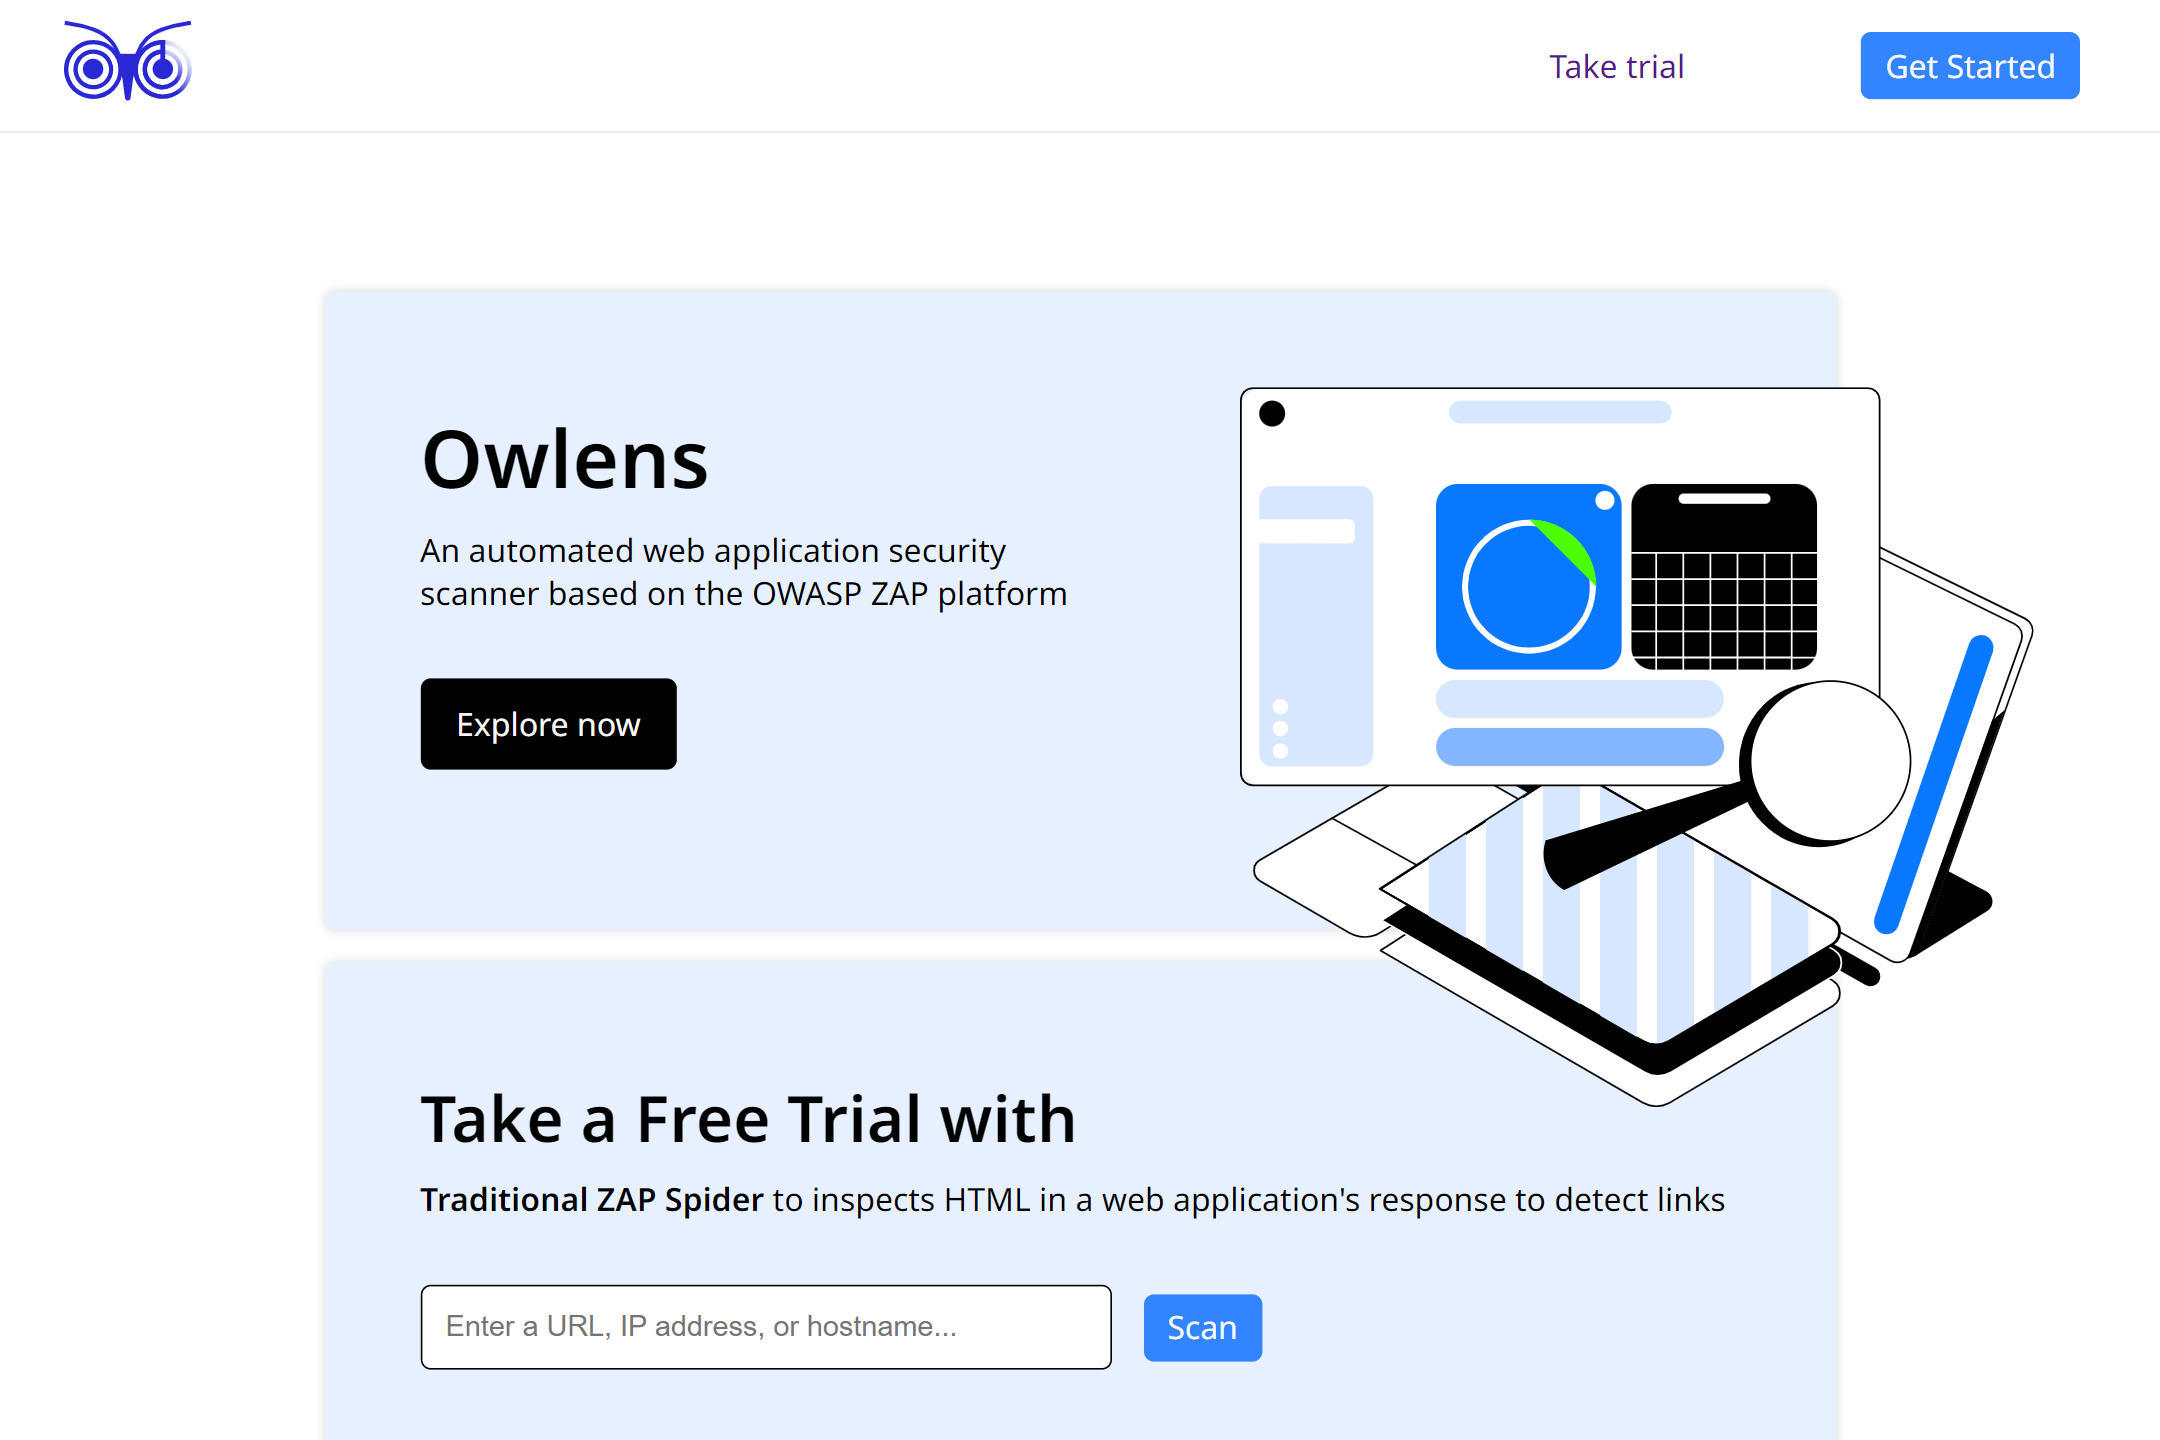
\includegraphics[width=\textwidth]{applied-thesis-chapters/chapter-6/Màn hình trang chủ.png}
      \caption{Màn hình trang chủ}
      \label{fig:ManHinhTrangChu}
\end{figure}

\begin{figure}[H]
      \centering
      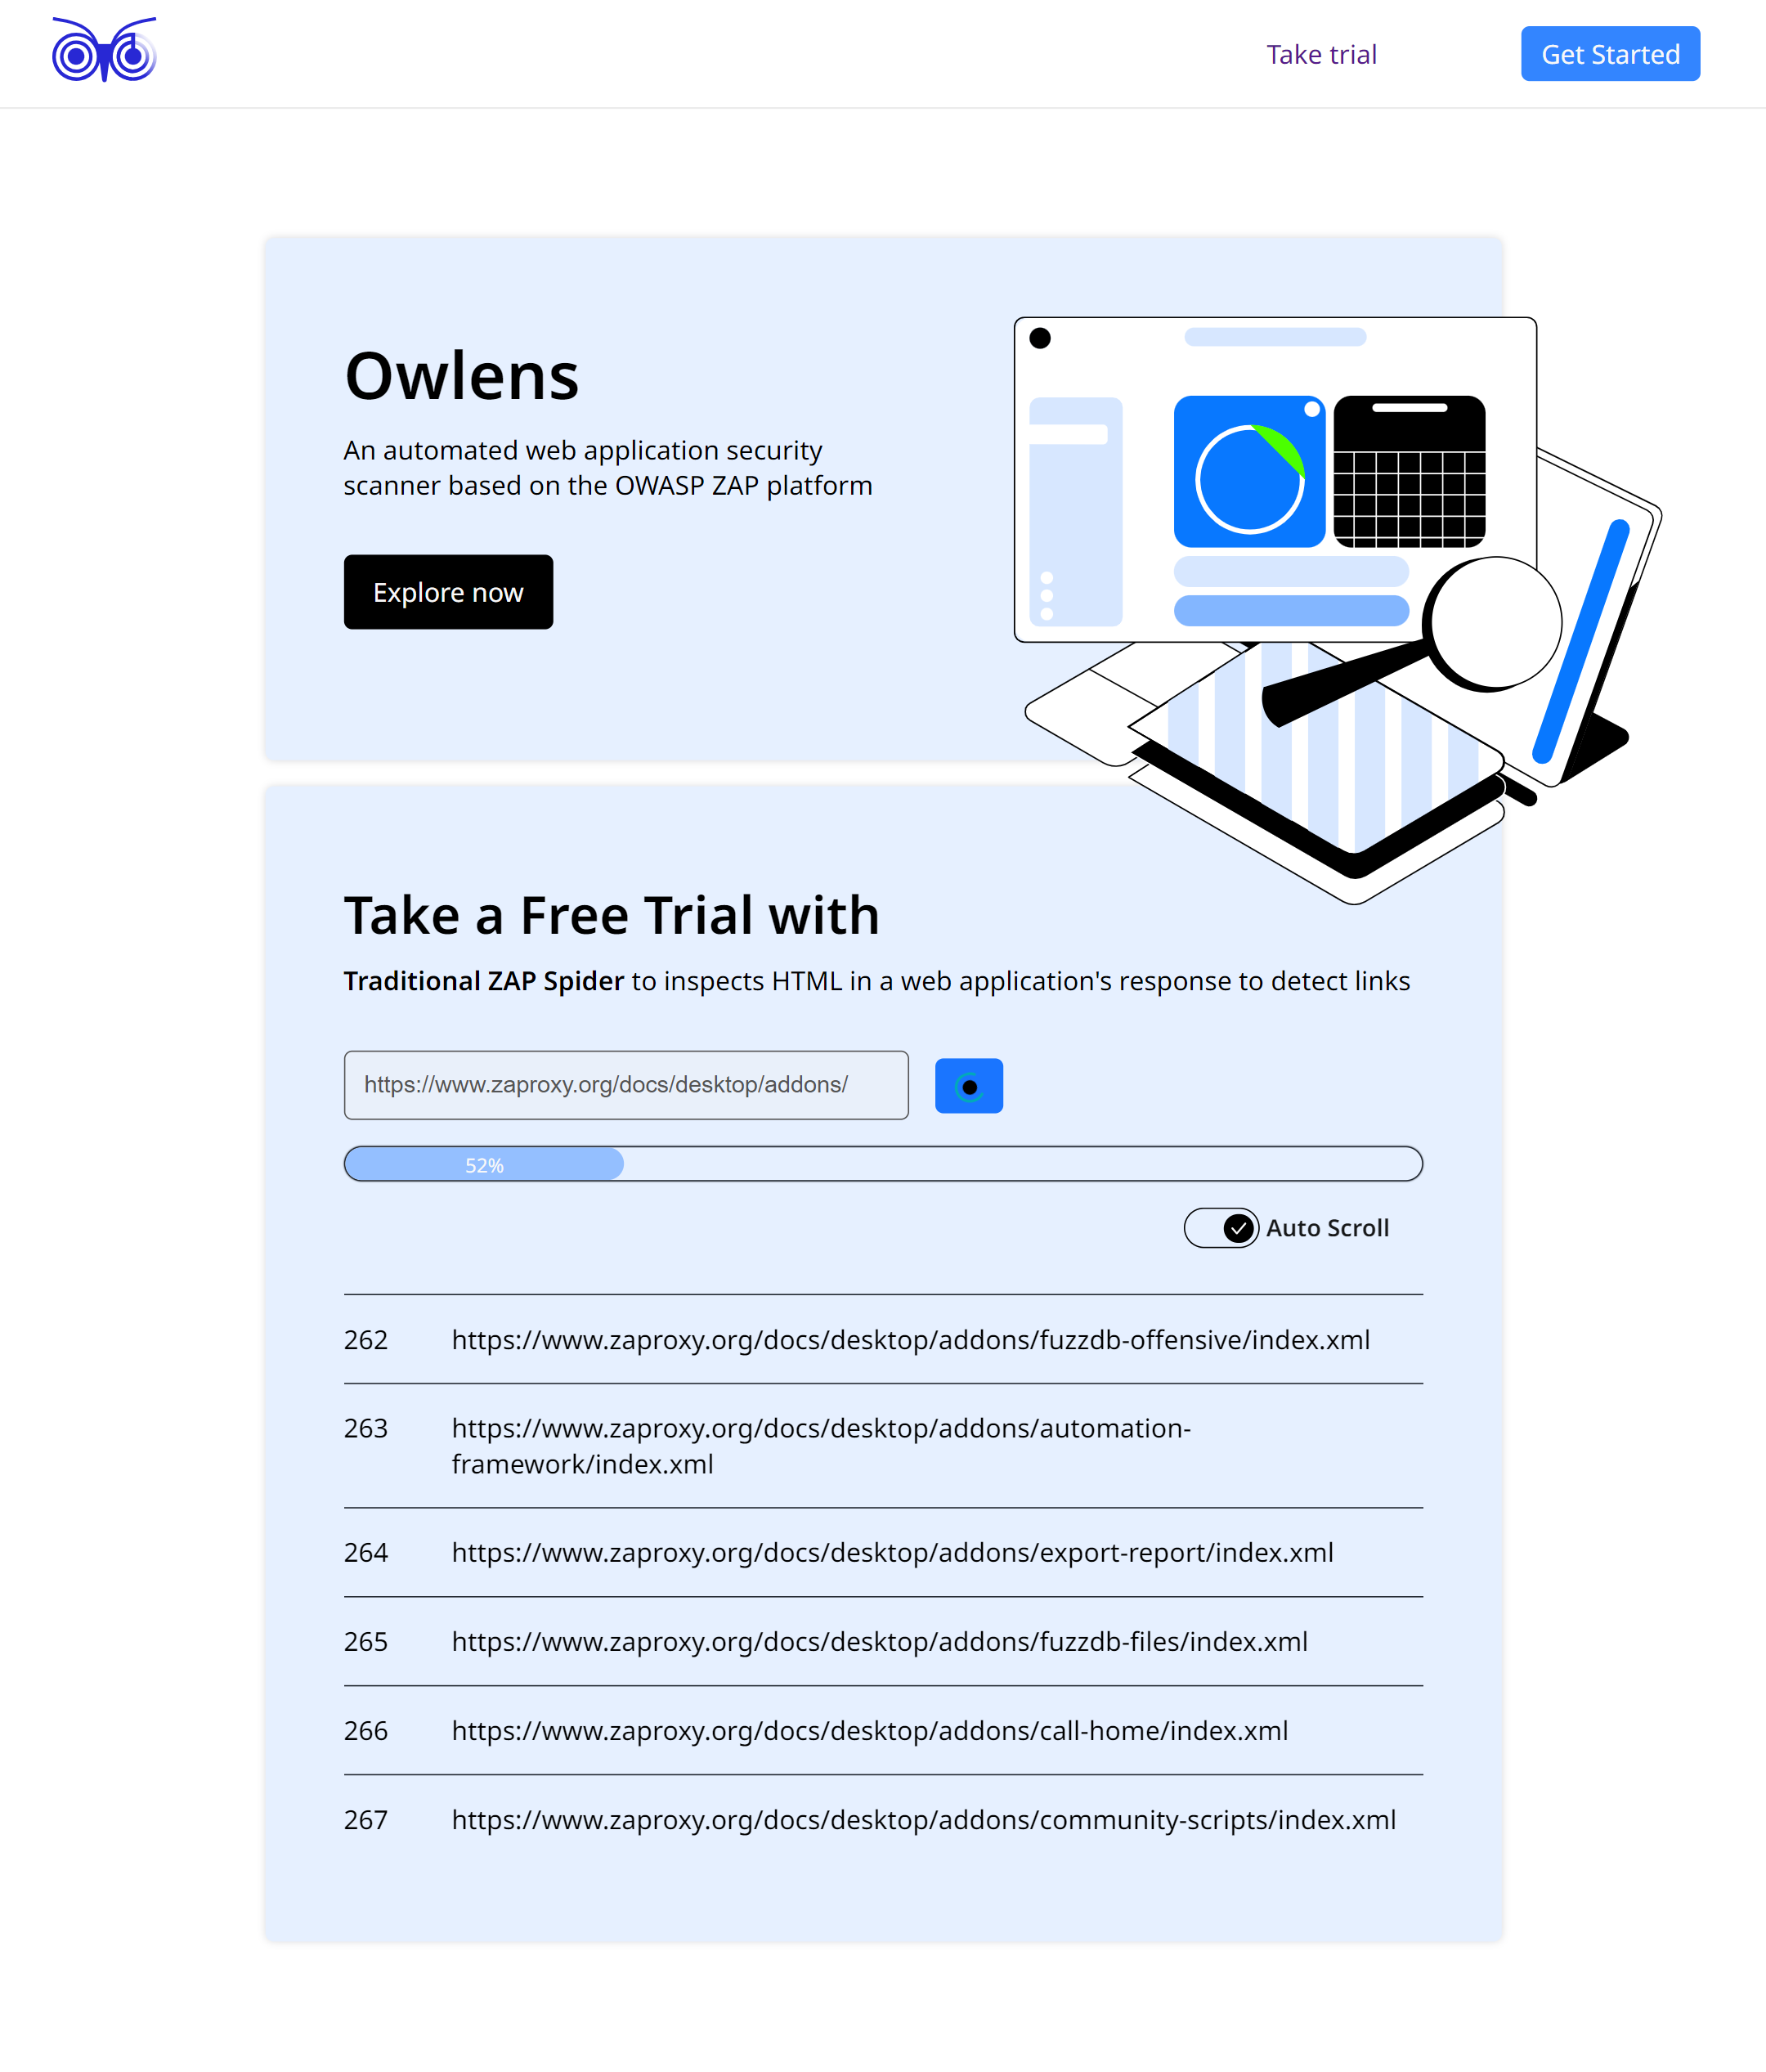
\includegraphics[width=\textwidth]{applied-thesis-chapters/chapter-6/Màn hình trang chủ và chức năng dùng thử 1.png}
      \caption{Màn hình trang chủ và chức năng dùng thử 1}
      \label{fig:ManHinhTrangChuVaChucNangDungThu1}
\end{figure}

\begin{figure}[H]
      \centering
      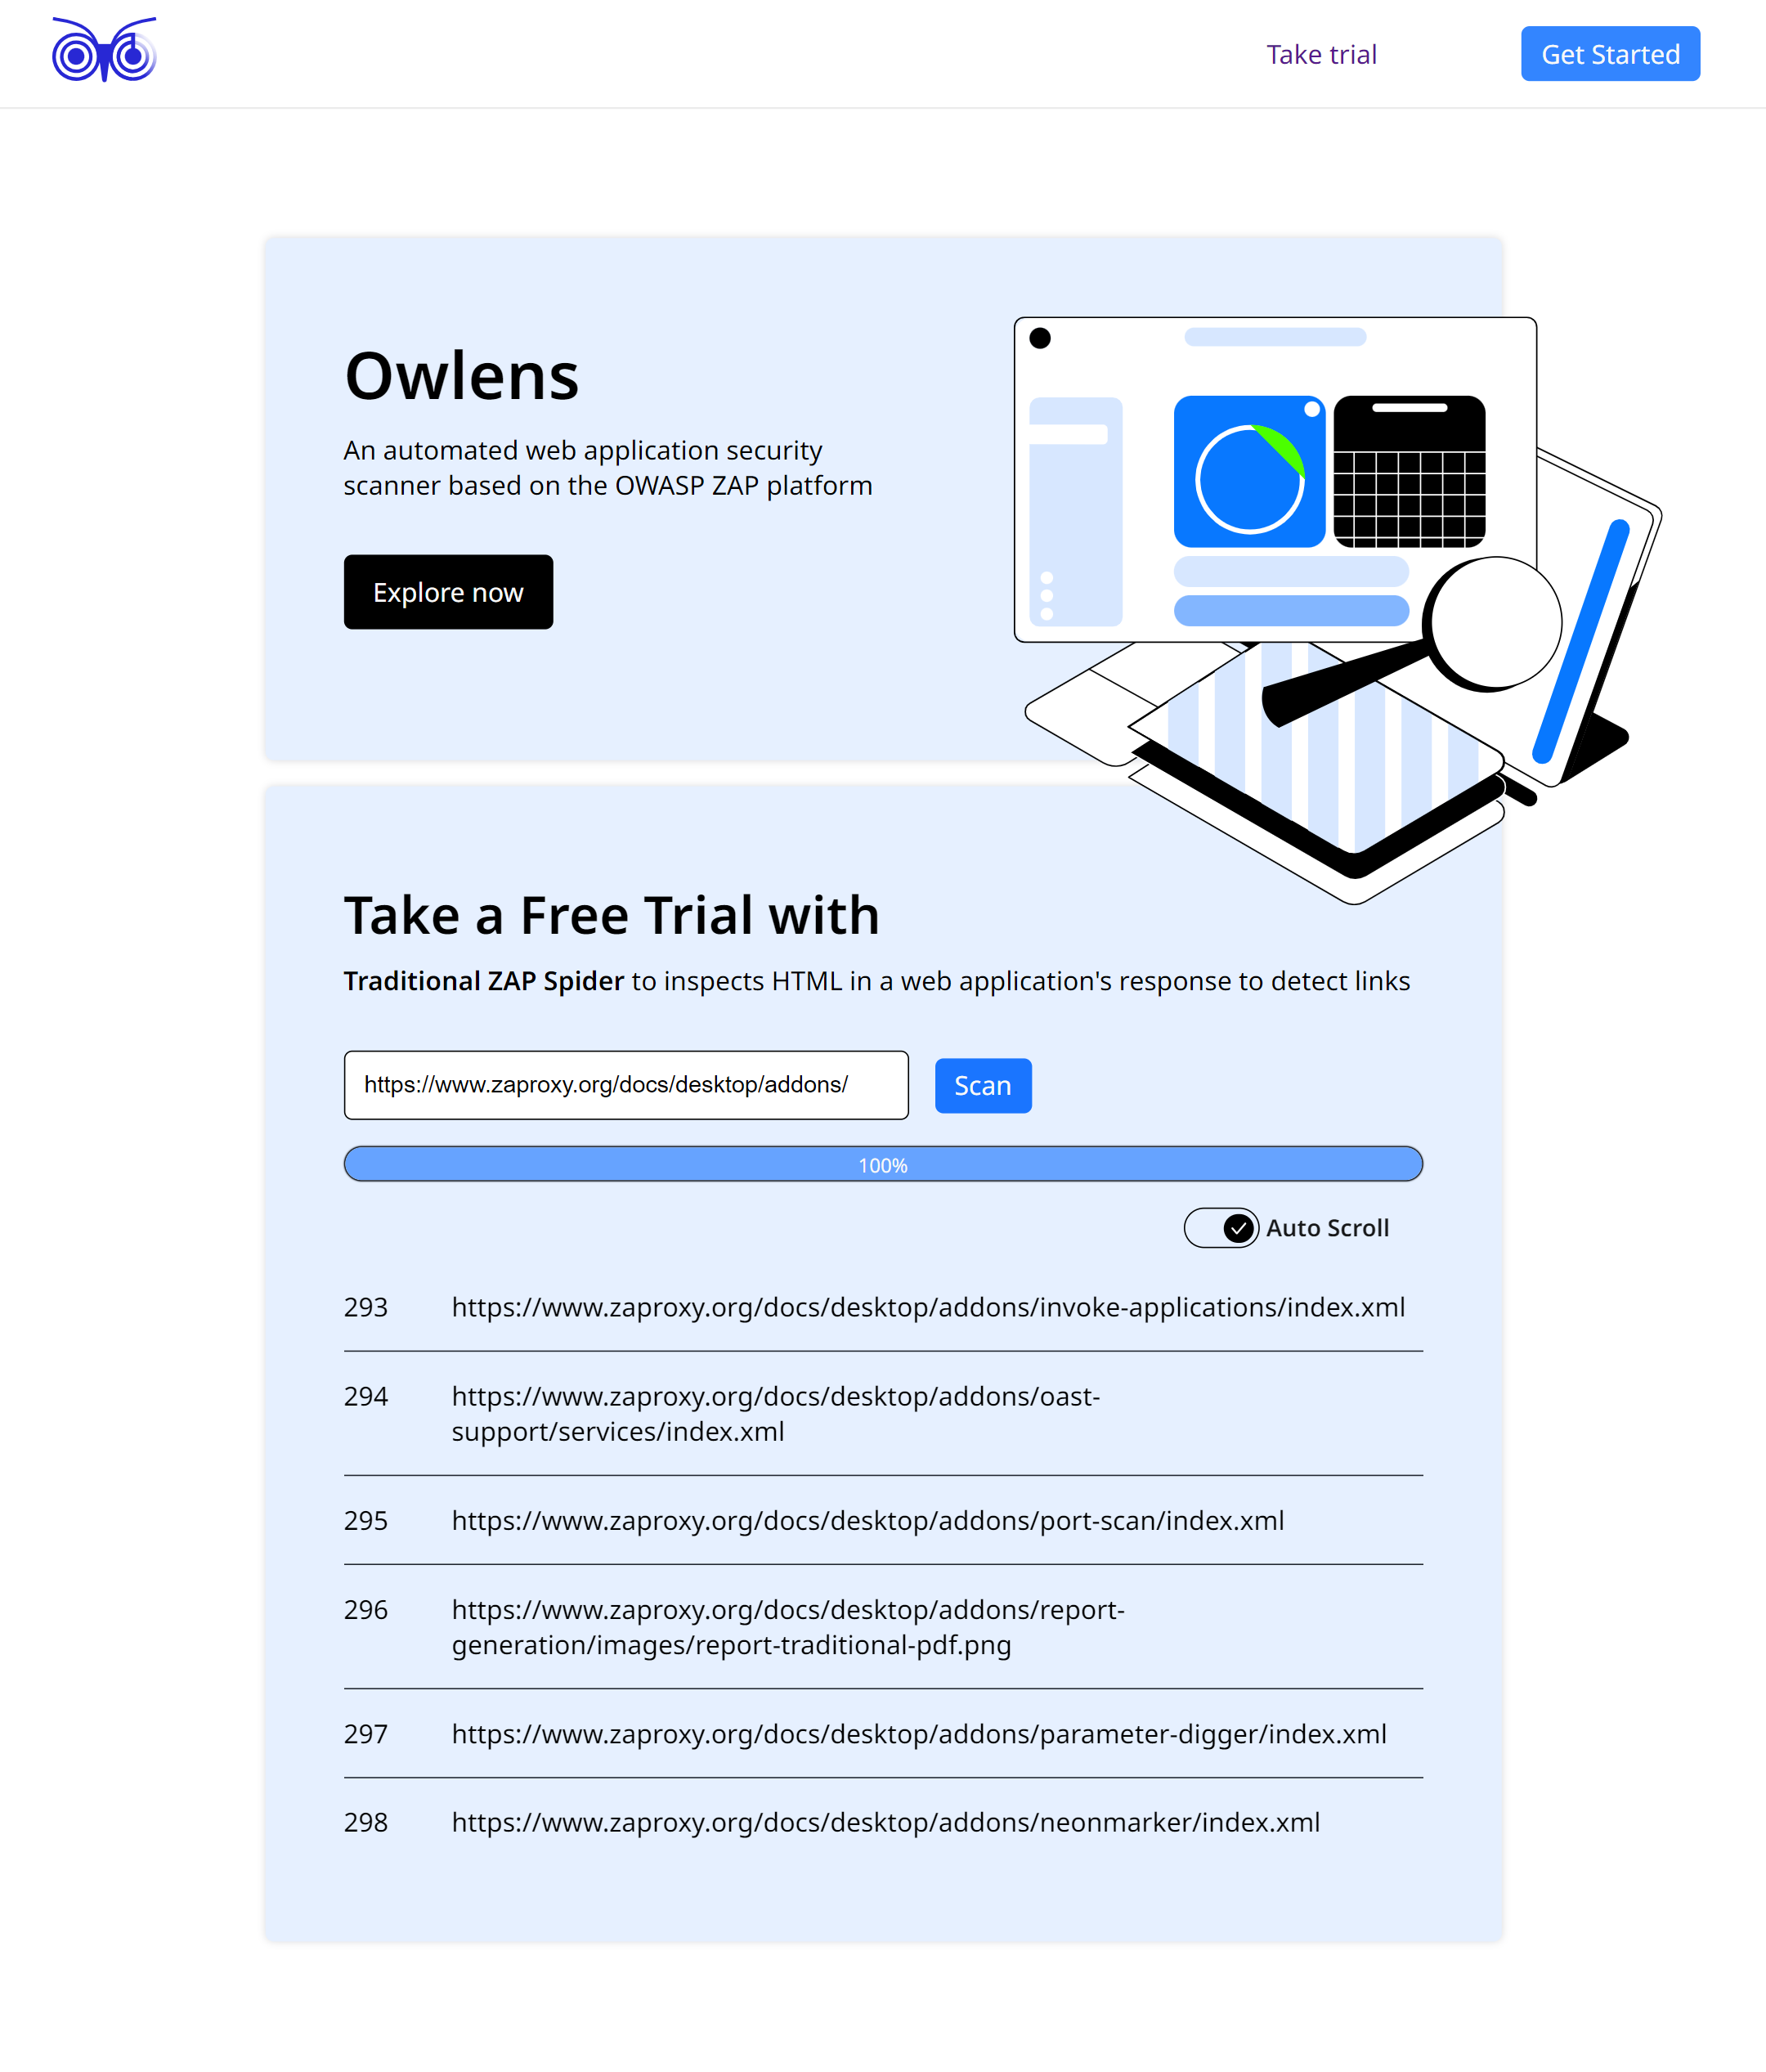
\includegraphics[width=\textwidth]{applied-thesis-chapters/chapter-6/Màn hình trang chủ và chức năng dùng thử 2.png}
      \caption{Màn hình trang chủ và chức năng dùng thử 2}
      \label{fig:ManHinhTrangChuVaChucNangDungThu2}
\end{figure}

\myparagraph{Trang đăng ký / đăng nhập}
\tab \tab Ở màn hình đăng nhập như hình \textit{\ref{fig:ManHinhTrangDangKyDangNhap} \nameref{fig:ManHinhTrangDangKyDangNhap}}, người dùng có thể thực hiện đăng ký / đăng nhập vào ứng dụng web bằng tài khoản Google.
Các trạng thái của quá trình đăng ký / đăng nhập cũng sẽ được thể hiện rõ ràng ở màn hình này.

\begin{figure}[H]
      \centering
      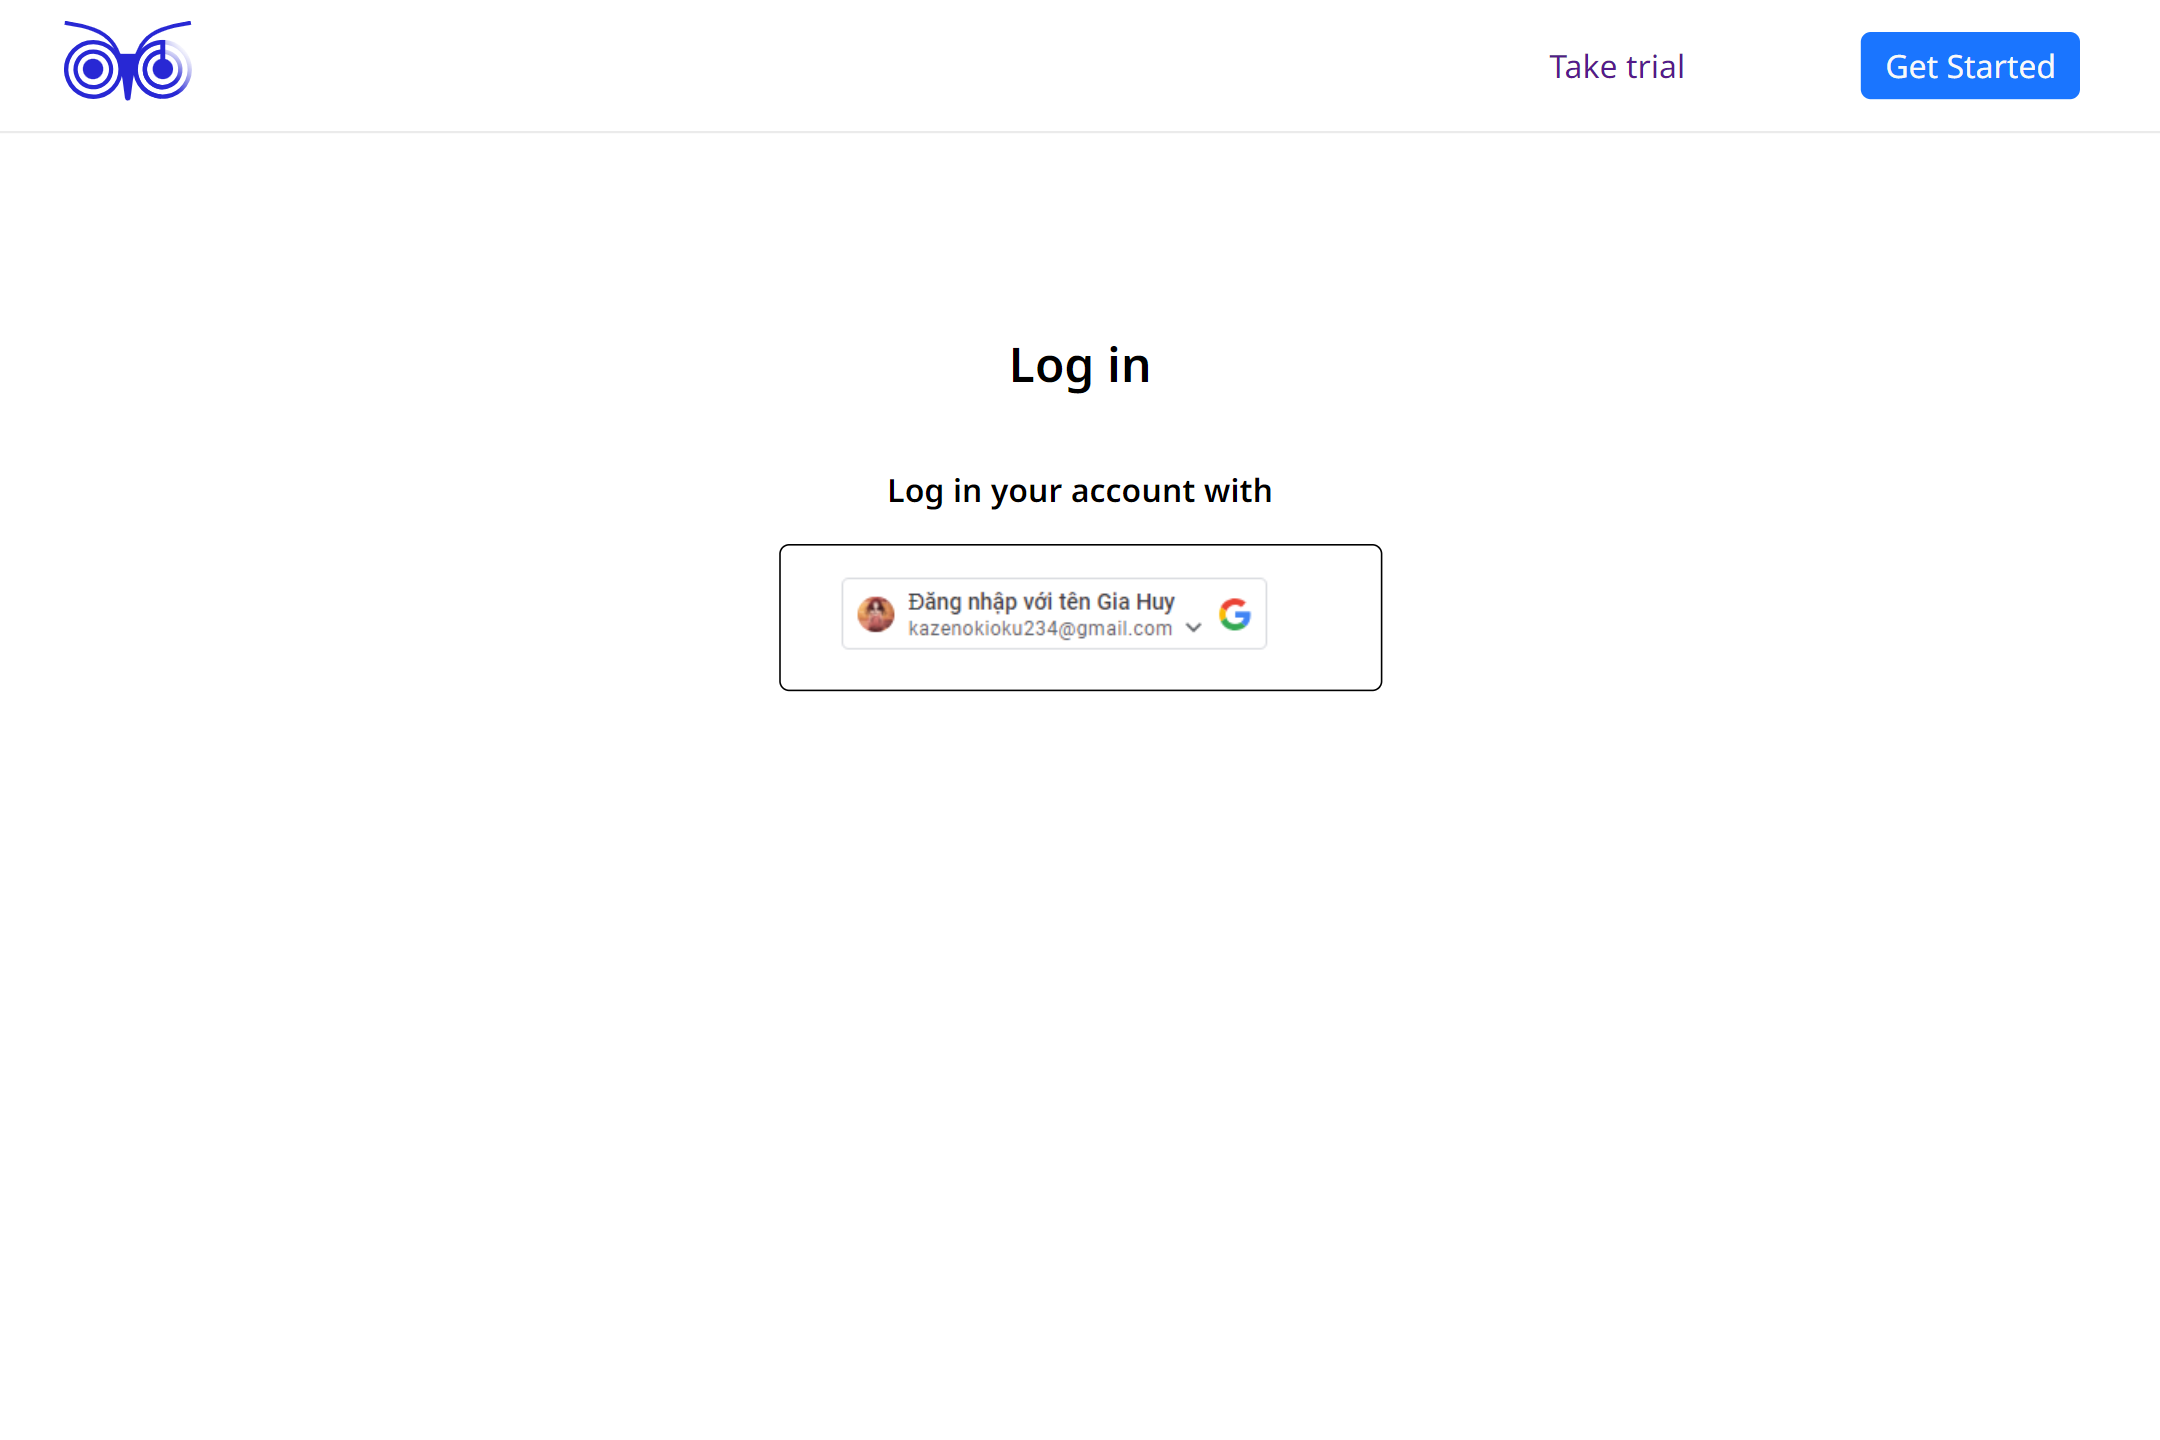
\includegraphics[width=\textwidth]{applied-thesis-chapters/chapter-6/Màn hình trang đăng nhập đăng ký.png}
      \caption{Màn hình trang đăng ký / đăng nhập}
      \label{fig:ManHinhTrangDangKyDangNhap}
\end{figure}

\subsection{Các màn hình bên trong ứng dụng}

\tab Sau khi đăng nhập thành công, người dùng sẽ truy cập vào được màn hình điều khiển ứng dụng.
Màn hình điều khiển ứng dụng được chia làm 5 phần chính Bảng điều khiển (Dashboard), Quản lý mục tiêu (Targets), Quản lý phiên quét (Results), Tạo phiên quét (New scan) và Cài đặt (Settings).

\myparagraph{Bảng điều khiển (Dashboard)}
\tab \tab Hình \textit{\ref{fig:ManHinhDashboard} \nameref{fig:ManHinhDashboard}} thể hiện giao diện phần Dashboard.
Màn hình Dashboard gồm hai phần thông tin là thông tin của hai phần Targets và Results.

\begin{figure}[H]
      \centering
      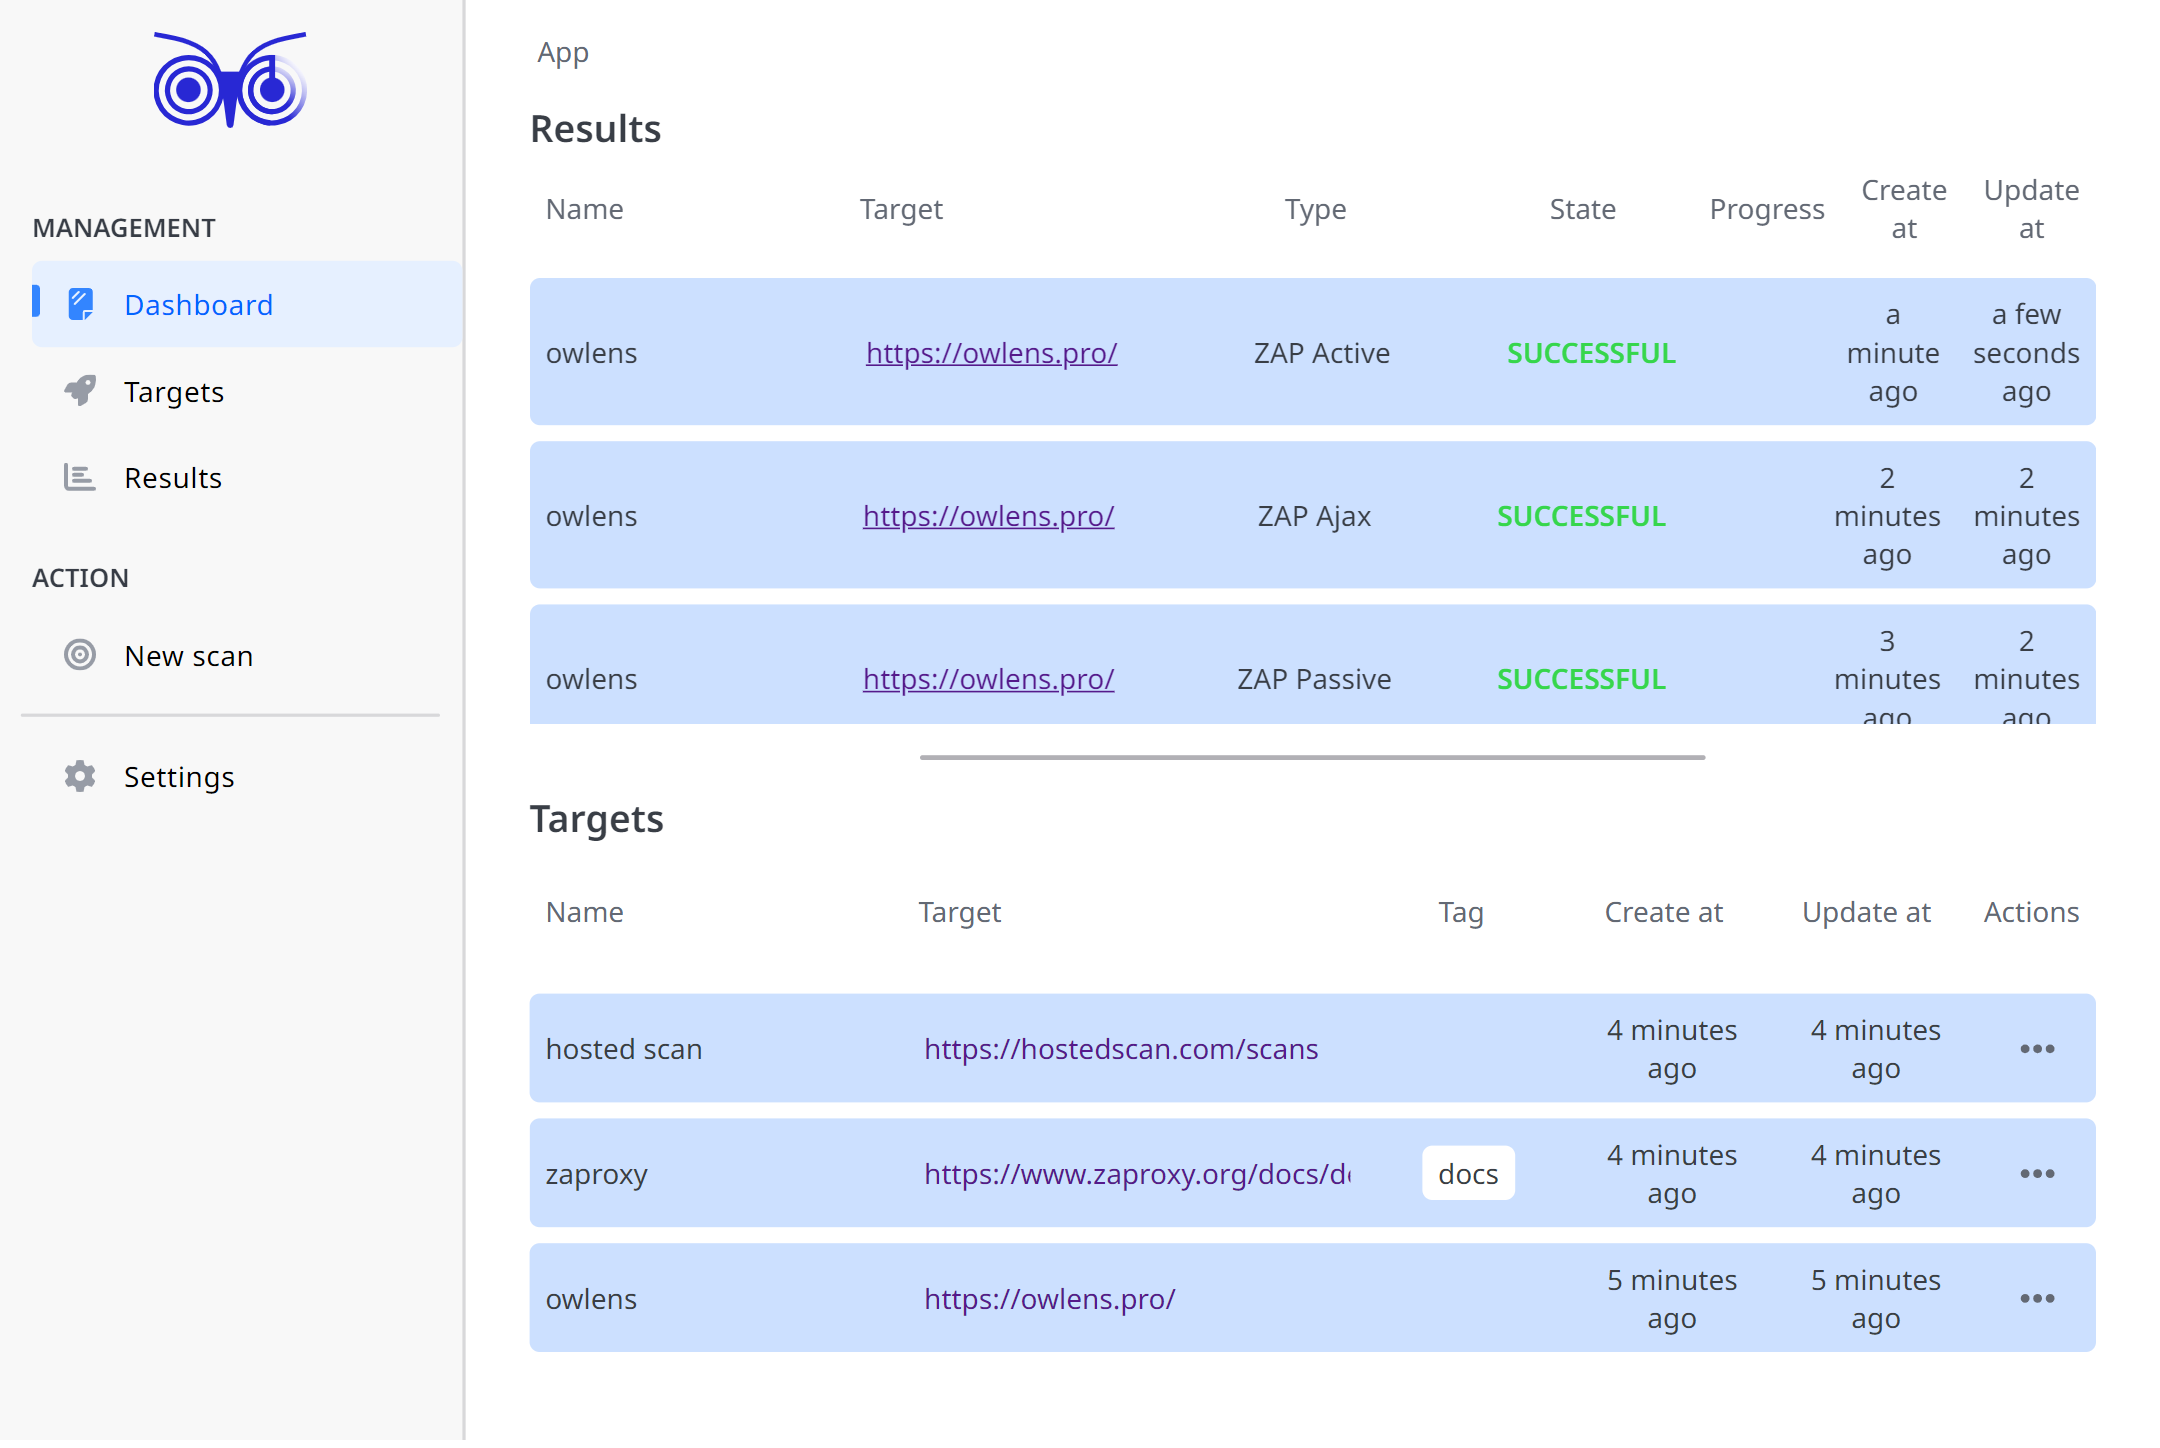
\includegraphics[width=\textwidth]{applied-thesis-chapters/chapter-6/Màn hình Dashboard.png}
      \caption{Màn hình Dashboard}
      \label{fig:ManHinhDashboard}
\end{figure}

Người dùng có thể truy cập, sử dụng nhanh các tác vụ mà không cần đi đến hai màn hình điều khiển cụ thể của từng phần.
Trong Dashboard, thứ tự hiển thị trên dưới của hai phần Results và Targets sẽ thay đổi theo thời gian thay đổi dữ liệu nội tại của từng phần.
Ví dụ, nếu dữ liệu của Targets có thay đổi mới gần hơn Results thì phần Targets sẽ được hiển thị bên trên và ngược lại.

\myparagraph{Quản lý mục tiêu (Targets)}
\tab \tab Hình \textit{\ref{fig:ManHinhTargets} \nameref{fig:ManHinhTargets}} thể hiện giao diện phần Targets.
Màn hình Targets thể hiện thông tin và quản lý các mục tiêu.

\begin{figure}[H]
      \centering
      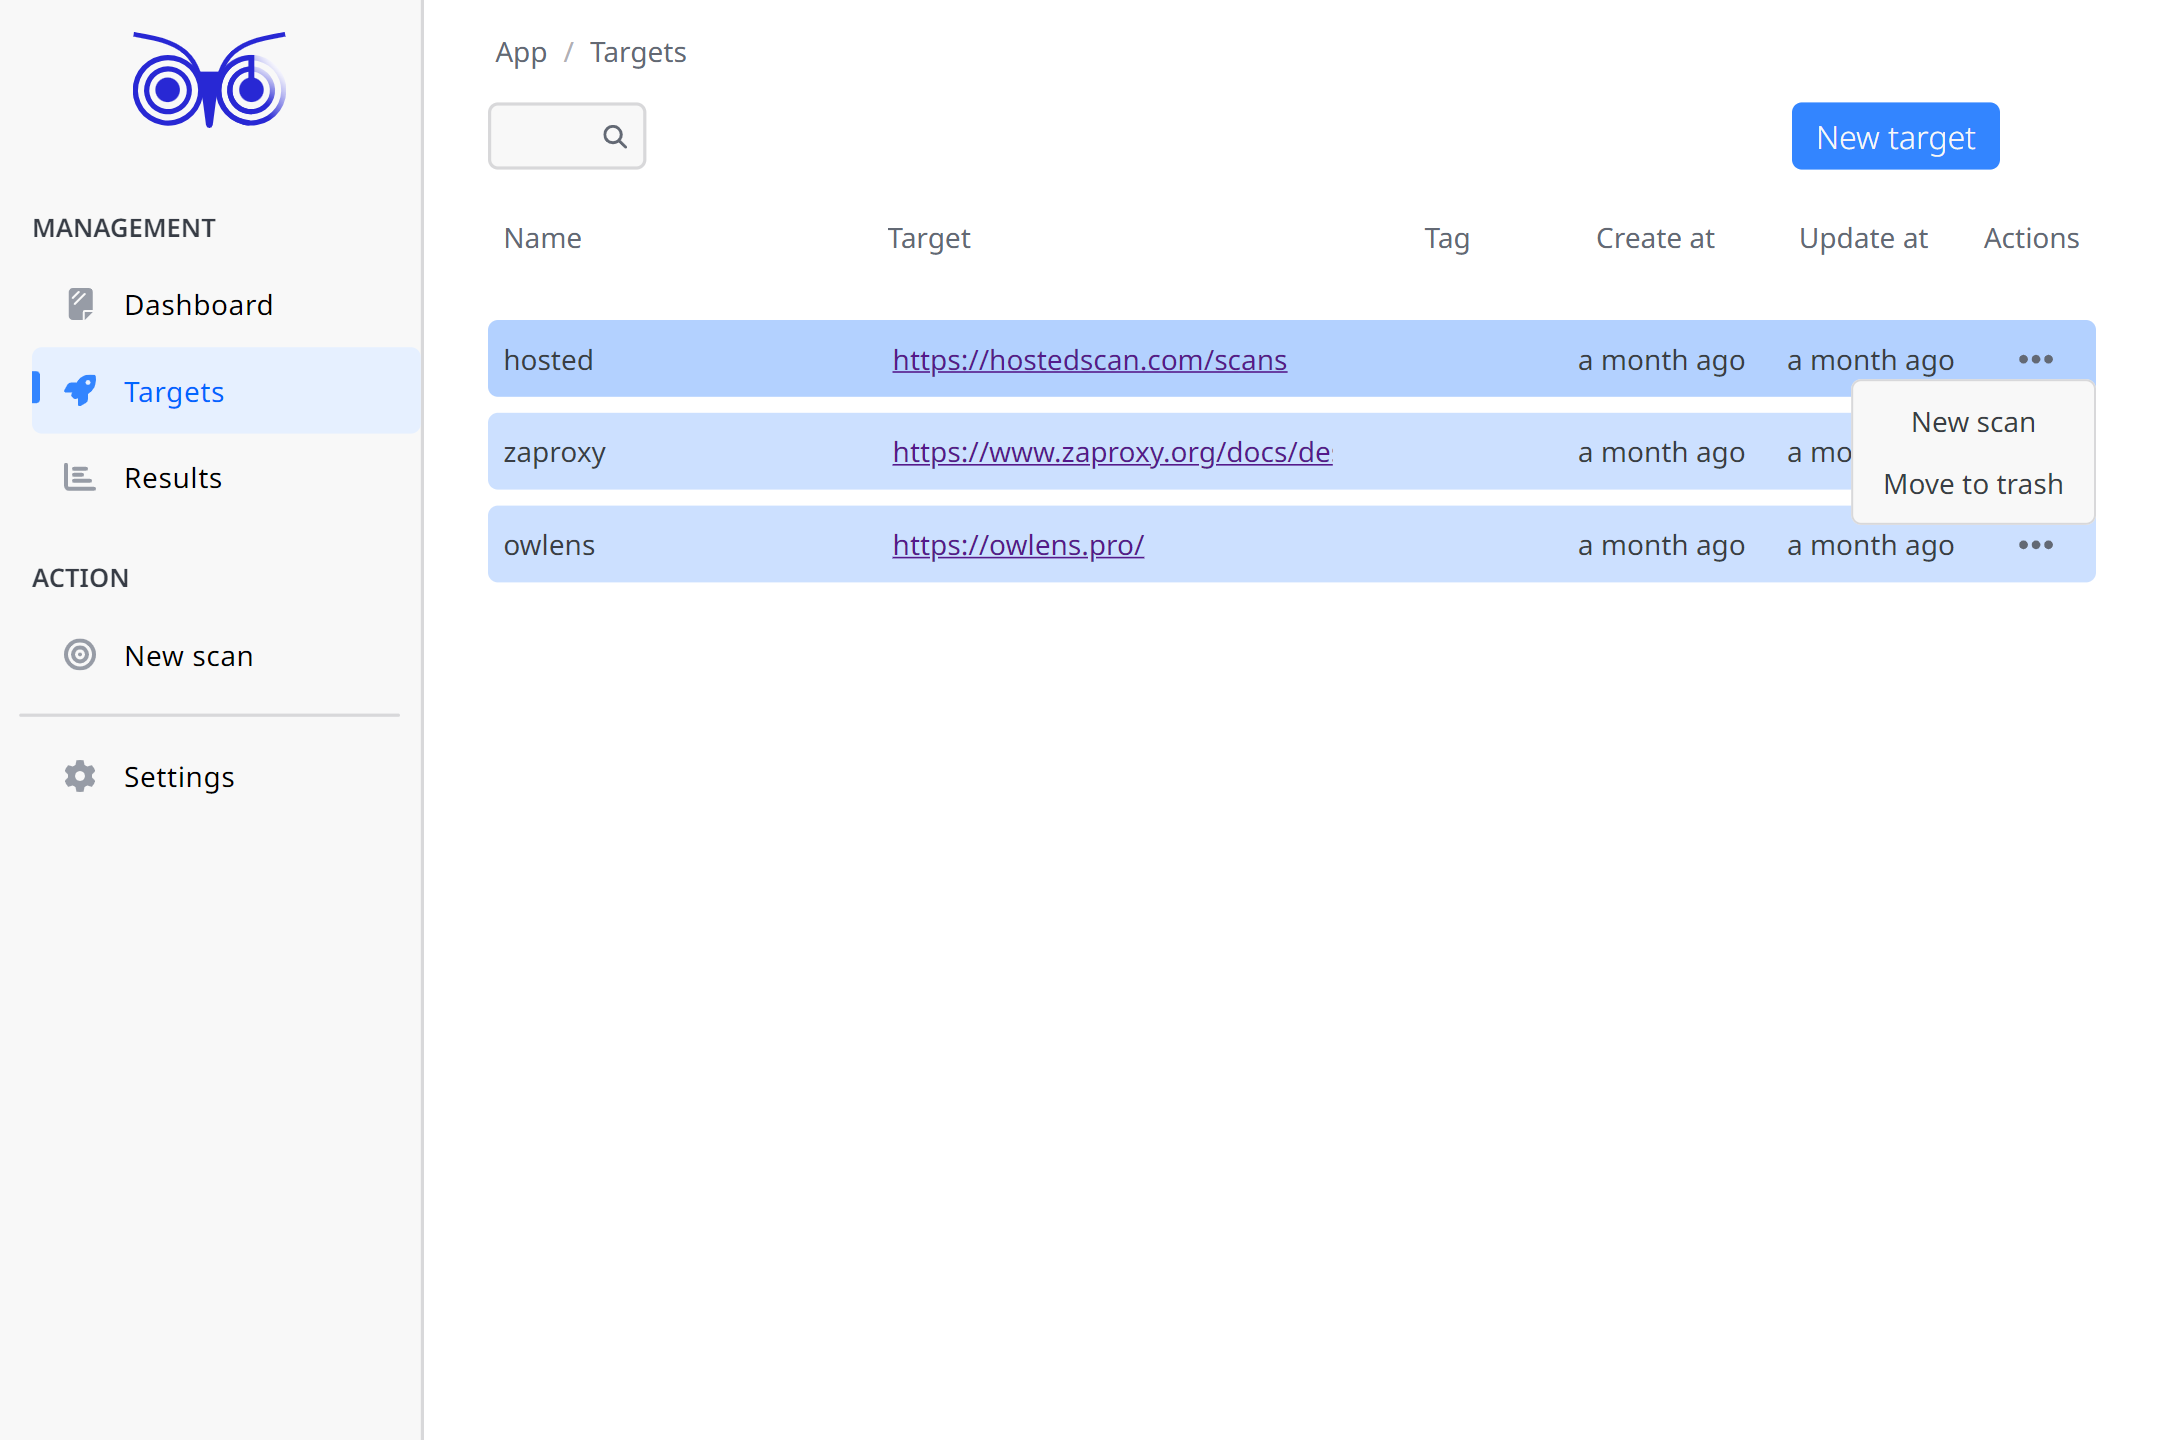
\includegraphics[width=\textwidth]{applied-thesis-chapters/chapter-6/Màn hình Targets.png}
      \caption{Màn hình Targets}
      \label{fig:ManHinhTargets}
\end{figure}

Người dùng có thể xóa mục tiêu và tạo mới phiên quét trong mỗi mục của mục tiêu.
Người dùng cũng thực hiện tạo mới mục tiêu ở đây.

Các hình \textit{\ref{fig:ManHinhTargetsVaThemMoiMucTieu1} \nameref{fig:ManHinhTargetsVaThemMoiMucTieu1}} 
và \textit{\ref{fig:ManHinhTargetsVaThemMoiMucTieu2} \nameref{fig:ManHinhTargetsVaThemMoiMucTieu2}} thể hiện giao diện các màn hình và cửa sổ trong quá trình tạo mới mục tiêu.

\begin{figure}[H]
      \centering
      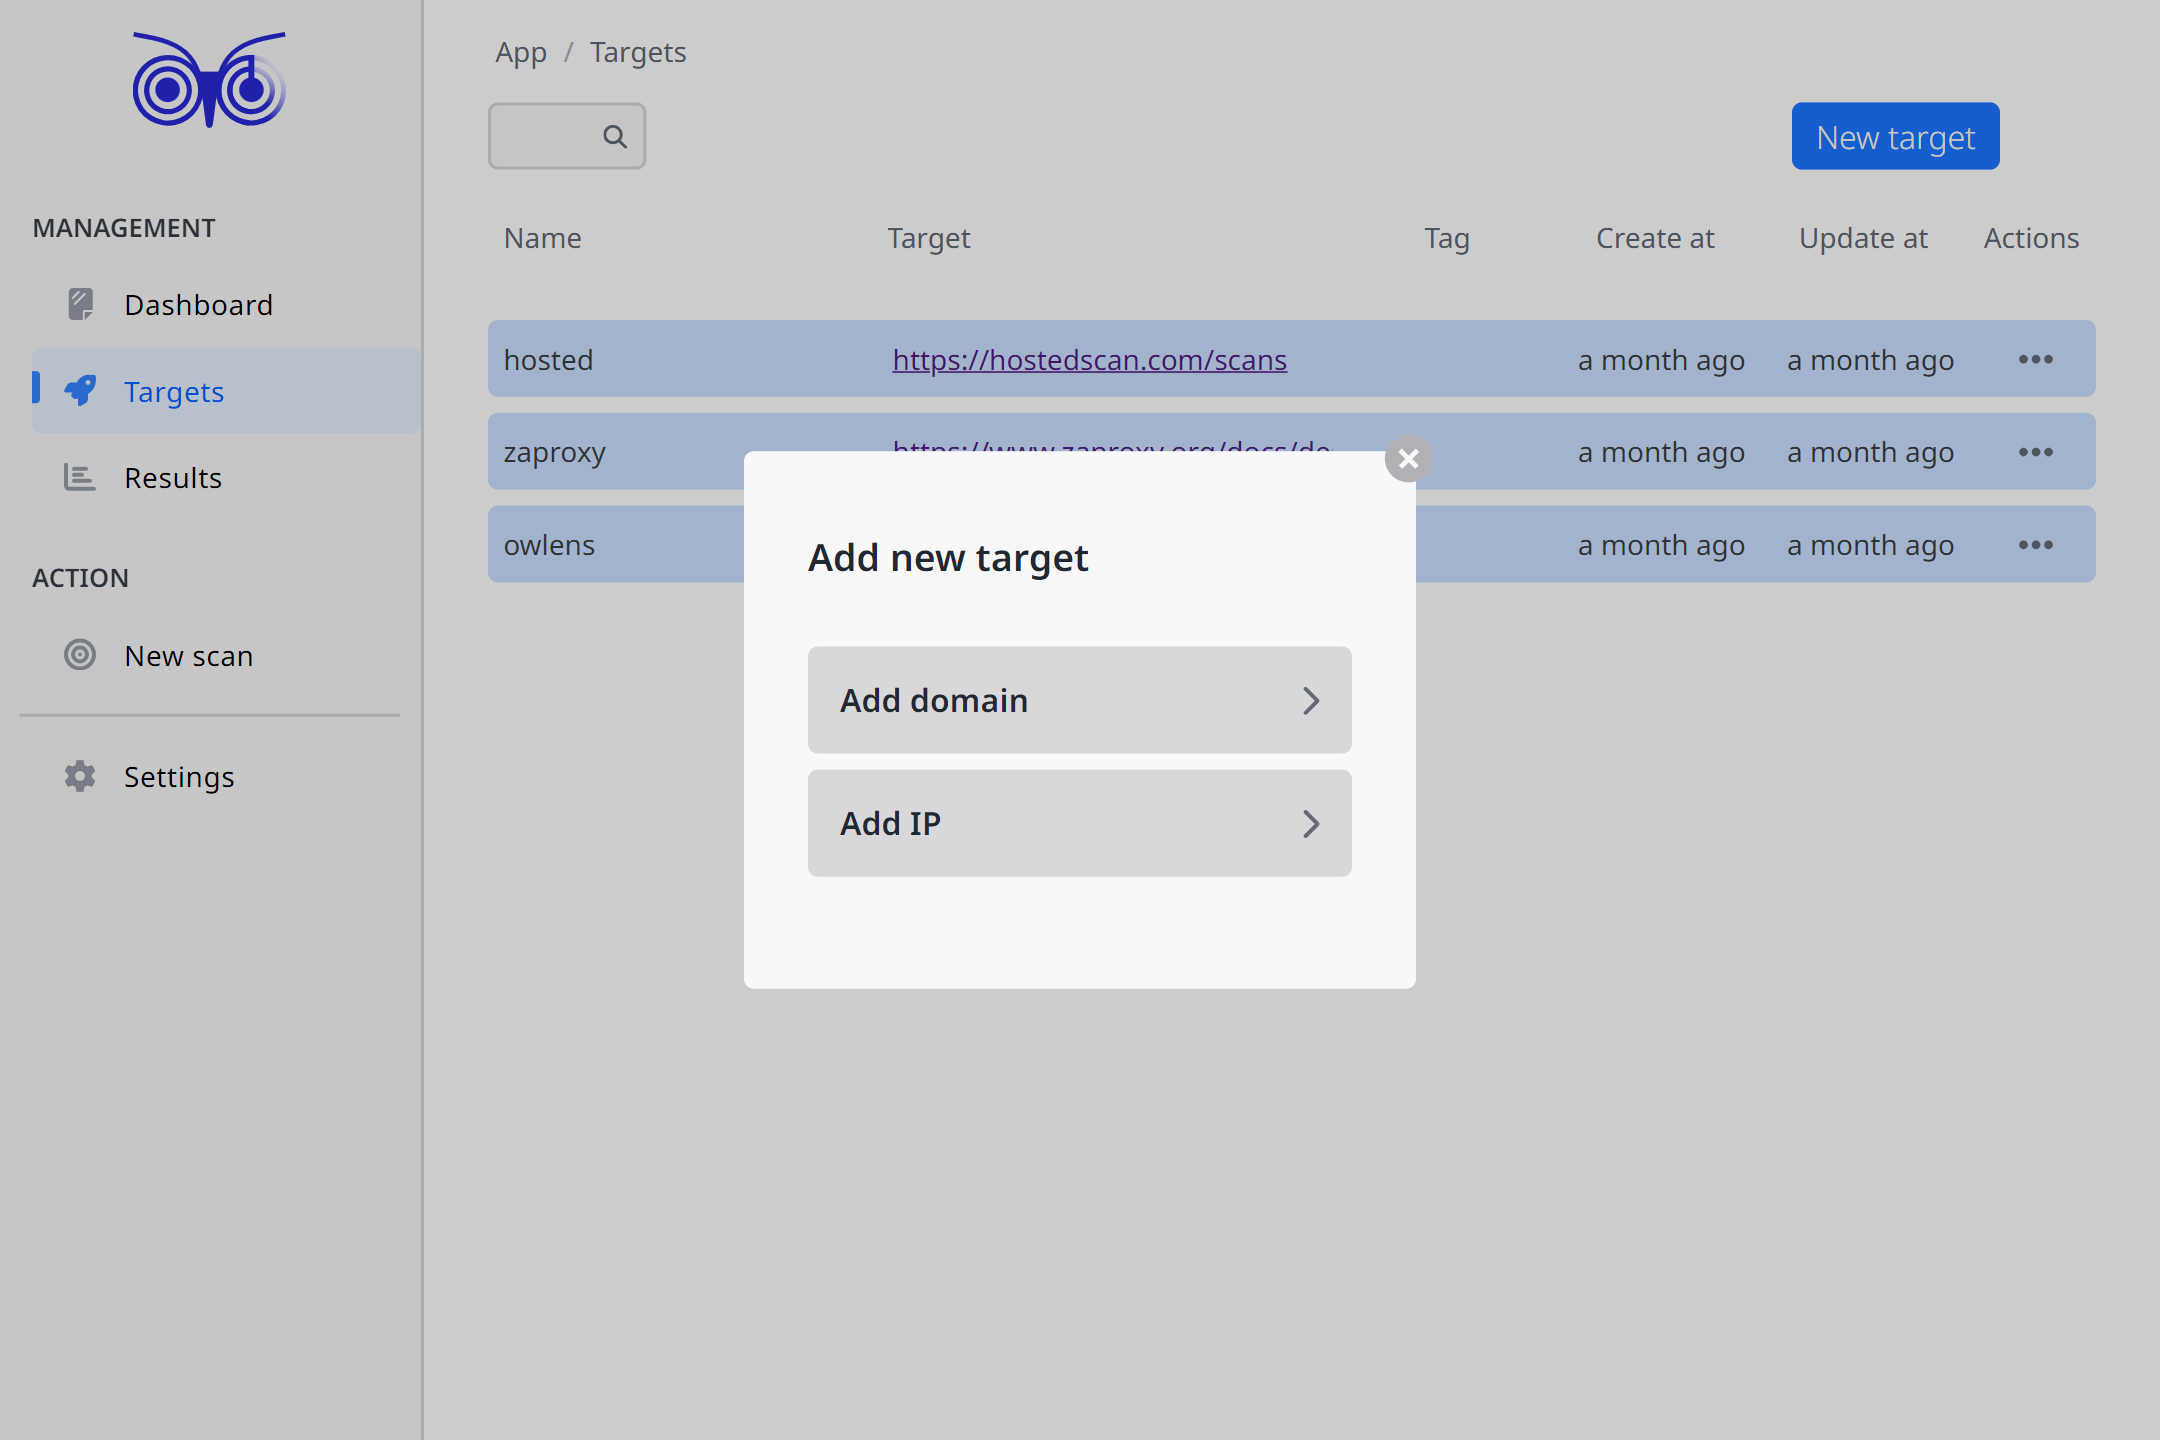
\includegraphics[width=\textwidth]{applied-thesis-chapters/chapter-6/Màn hình Targets và thêm mới mục tiêu 1.png}
      \caption{Màn hình Targets và thêm mới mục tiêu 1}
      \label{fig:ManHinhTargetsVaThemMoiMucTieu1}
\end{figure}

\begin{figure}[H]
      \centering
      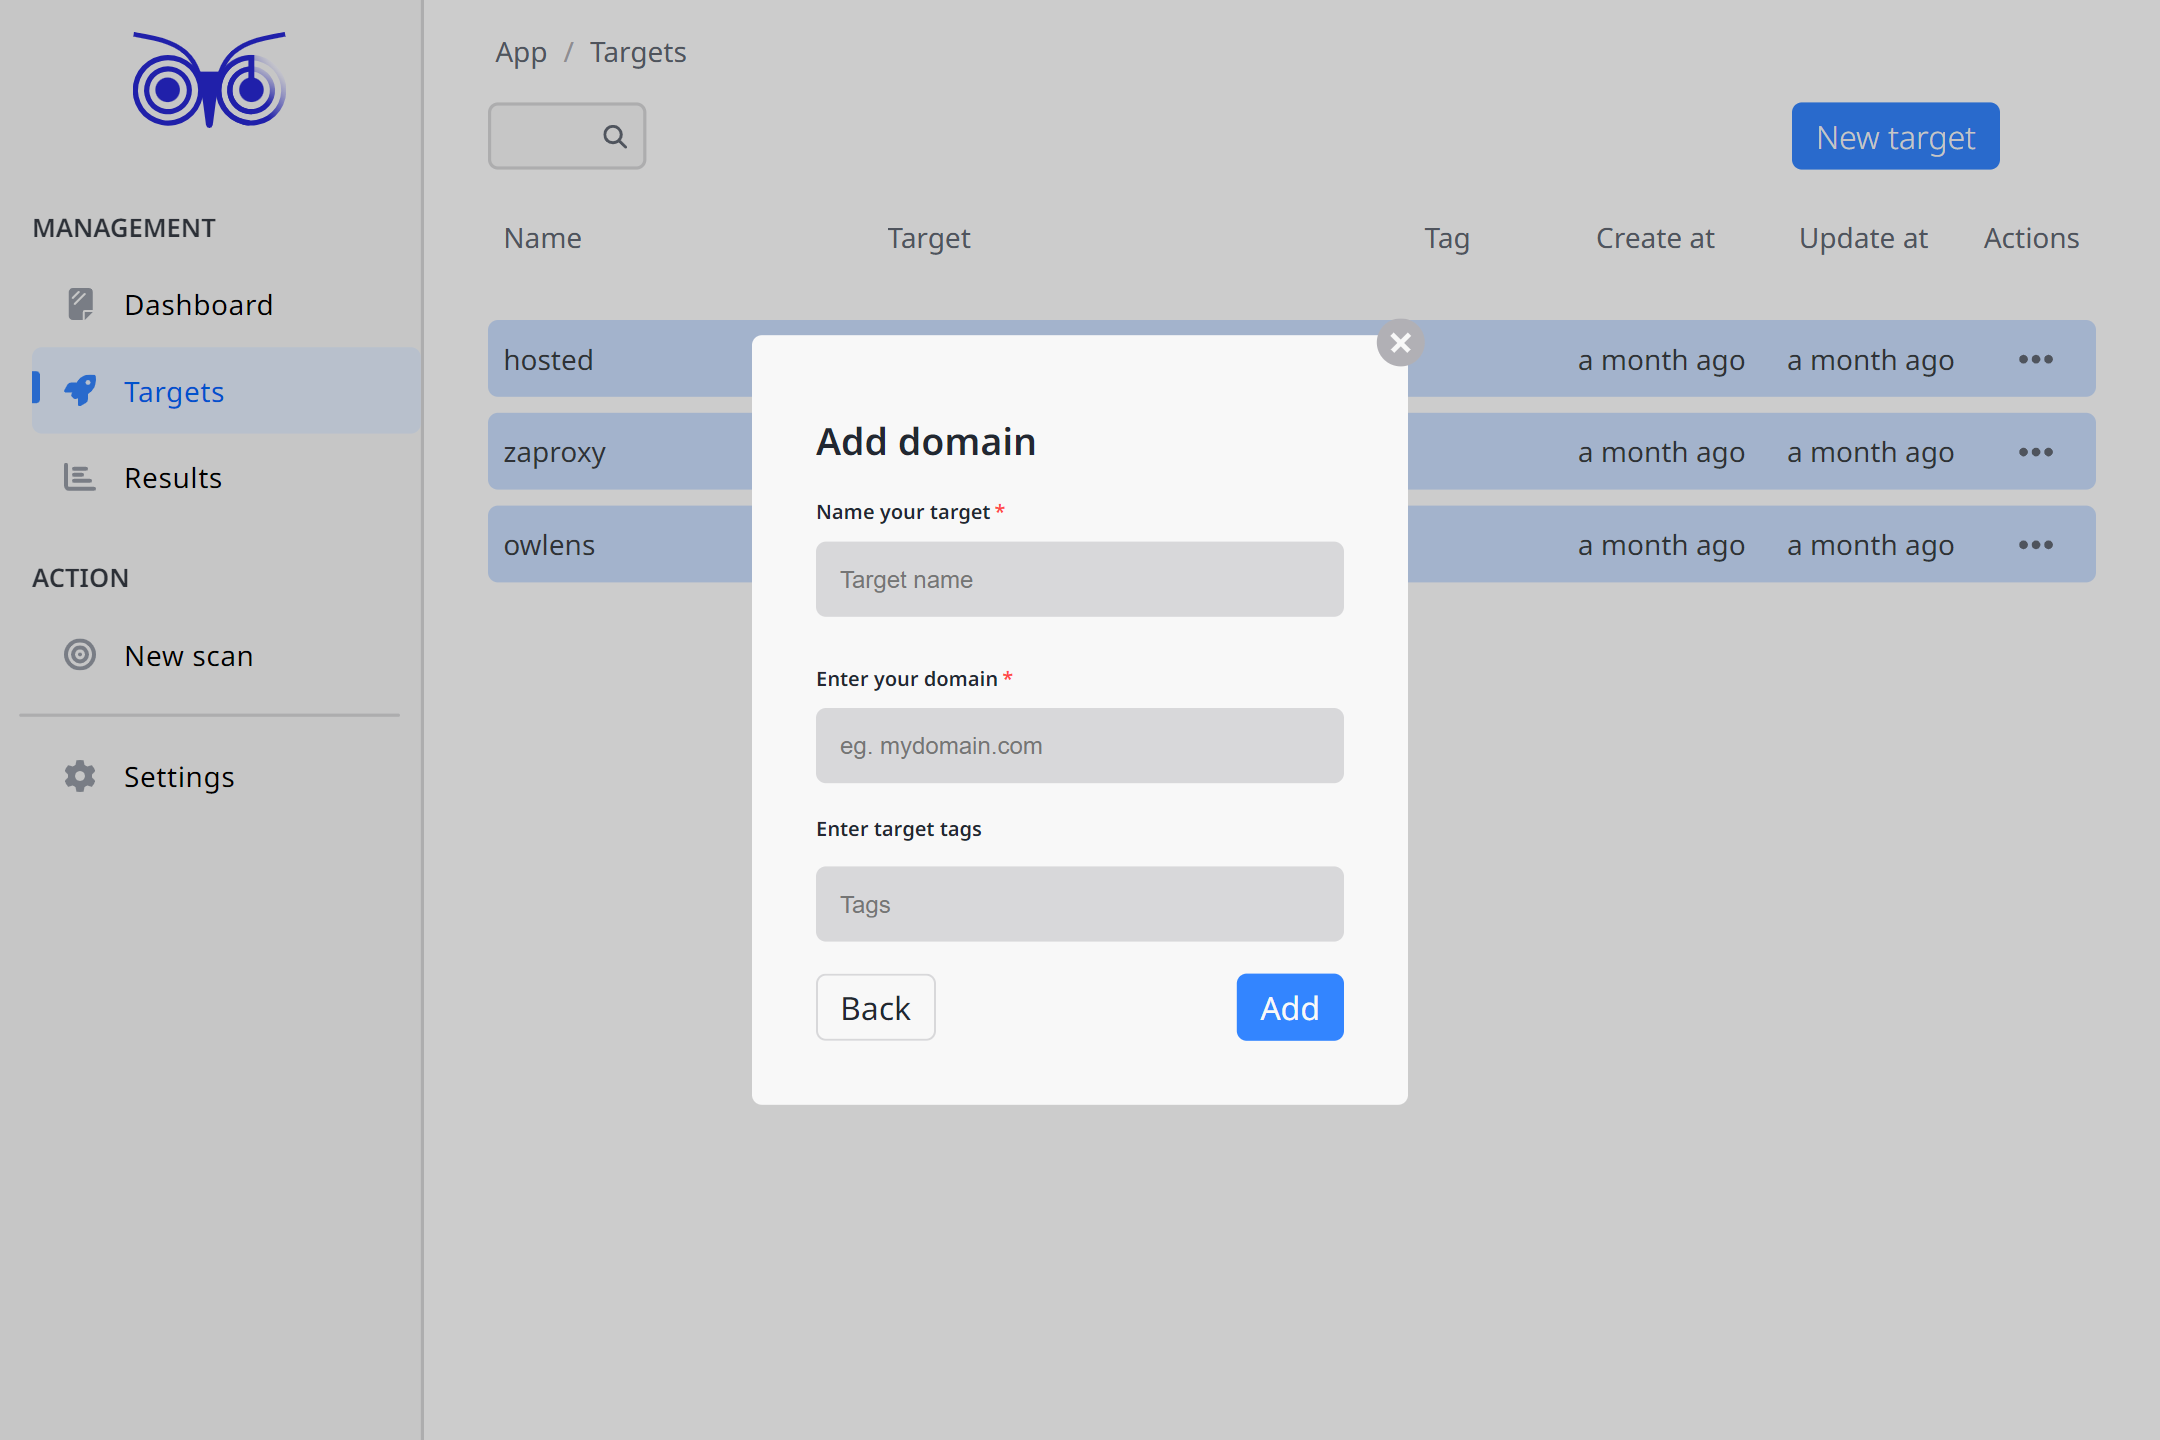
\includegraphics[width=\textwidth]{applied-thesis-chapters/chapter-6/Màn hình Targets và thêm mới mục tiêu 2.png}
      \caption{Màn hình Targets và thêm mới mục tiêu 2}
      \label{fig:ManHinhTargetsVaThemMoiMucTieu2}
\end{figure}

Người dùng có thể tạo mới mục tiêu dạng URL hay IP, giao diện quá trình tạo mới mục tiêu dạng IP cũng tương tự khi thực hiện với URL.
Các thông báo ngoại lệ trong quá trình thêm mới mục tiêu được thể hiện trên cửa sổ thêm mới của màn hình ở hình \textit{\ref{fig:ManHinhTargetsVaThemMoiMucTieu2} \nameref{fig:ManHinhTargetsVaThemMoiMucTieu2}}.

\myparagraph{Quản lý phiên quét (Results)}
\tab \tab Hình \textit{\ref{fig:ManHinhResults} \nameref{fig:ManHinhResults}} thể hiện giao diện phần Results.
Màn hình Results thể hiện thông tin và trạng thái chung của các phiên quét.

\begin{figure}[H]
      \centering
      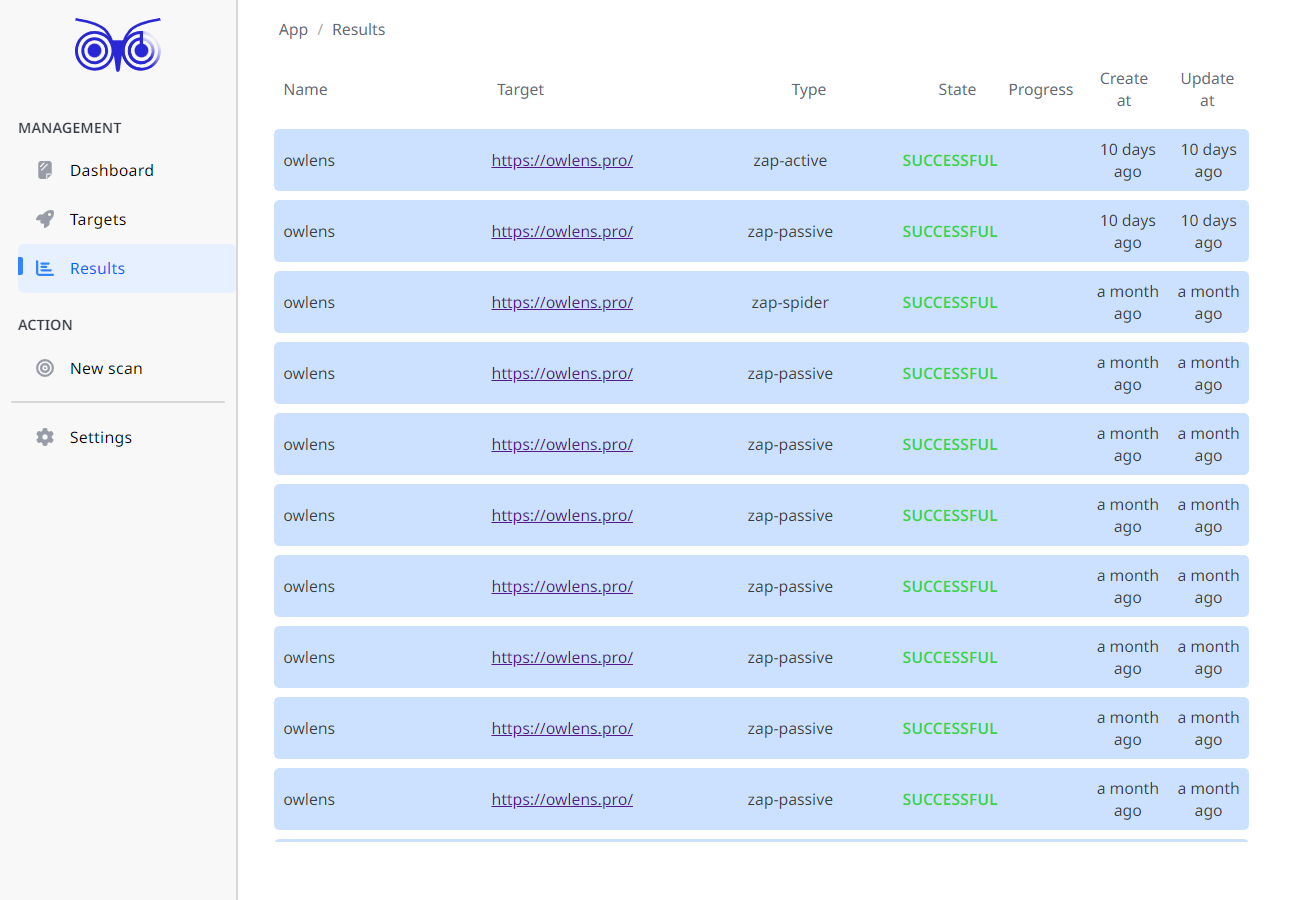
\includegraphics[width=\textwidth]{applied-thesis-chapters/chapter-6/Màn hình Results.png}
      \caption{Màn hình Results}
      \label{fig:ManHinhResults}
\end{figure}

Người dùng truy cập vào màn hình kết quả quét chi tiết của phiên quét bằng cách chọn vào mục của phiên quét.
Mỗi loại quét khác nhau sẽ có giao diện màn hình kết quả quét chi tiết khác nhau.

Các hình \textit{\ref{fig:ManHinhKetQuaQuetChiTietSpiderVaURLsInScope} \nameref{fig:ManHinhKetQuaQuetChiTietSpiderVaURLsInScope}} 
và \textit{\ref{fig:ManHinhKetQuaQuetChiTietSpiderVaURLsOutOfScope} \nameref{fig:ManHinhKetQuaQuetChiTietSpiderVaURLsOutOfScope}} 
thể hiện giao diện màn hình kết quả quét chi tiết của phiên quét loại Spider.

\begin{figure}[H]
      \centering
      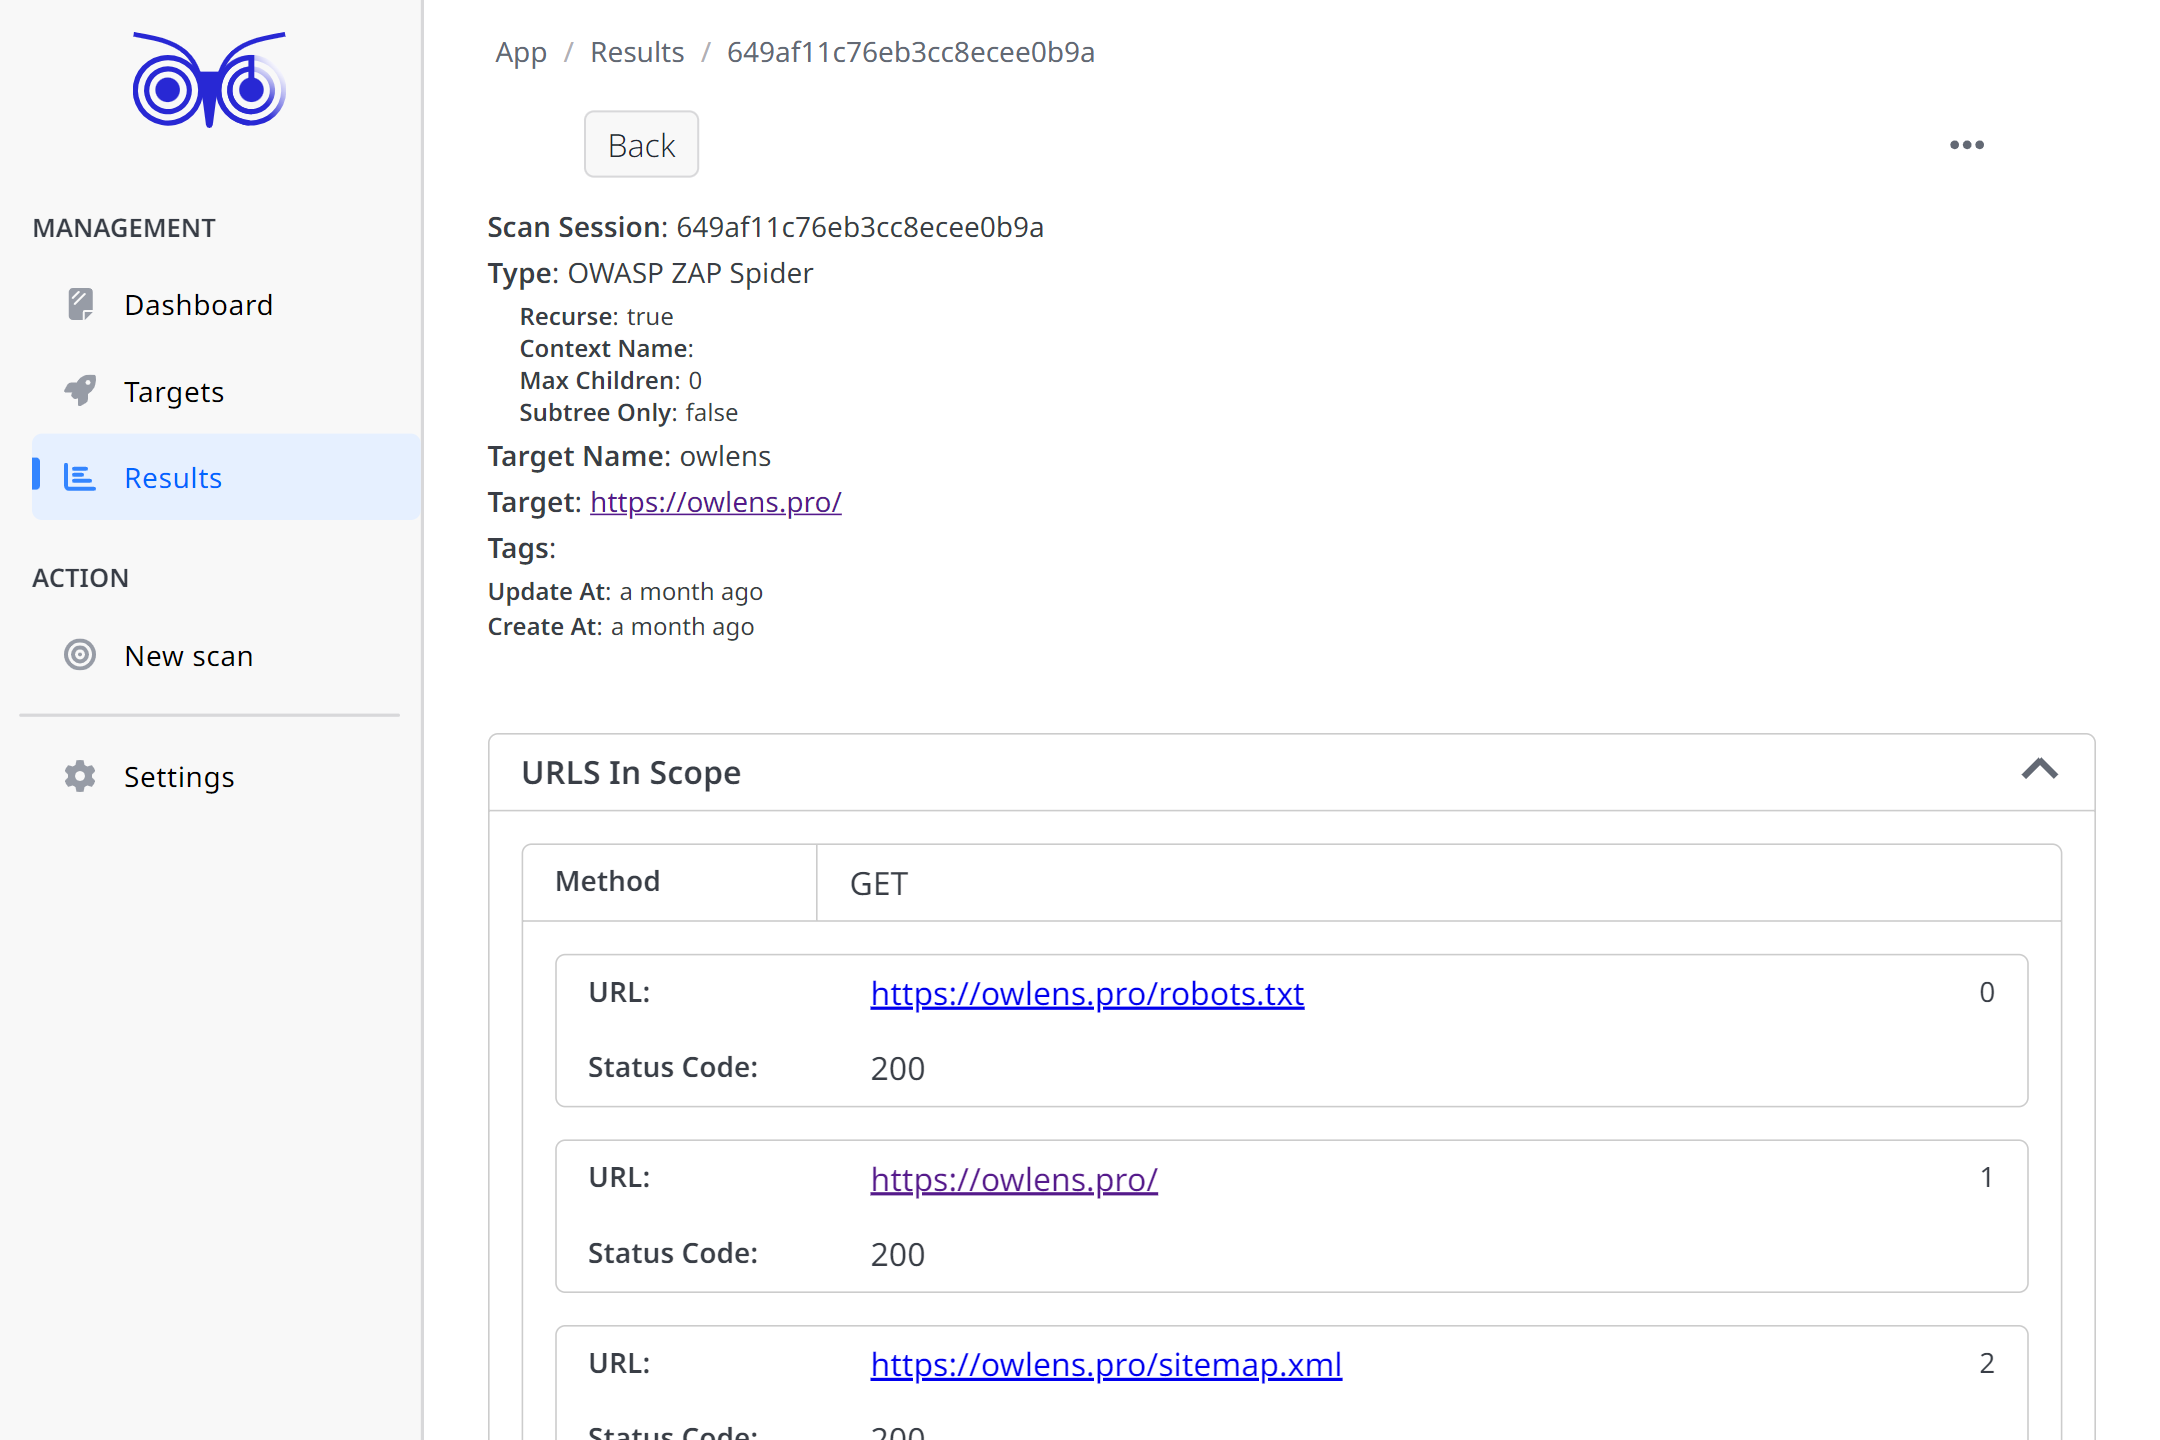
\includegraphics[width=\textwidth]{applied-thesis-chapters/chapter-6/Màn hình kết quả quét chi tiết Spider và bảng URLs In Scope.png}
      \caption{Màn hình kết quả quét chi tiết Spider và bảng URLs In Scope}
      \label{fig:ManHinhKetQuaQuetChiTietSpiderVaURLsInScope}
\end{figure}

\begin{figure}[H]
      \centering
      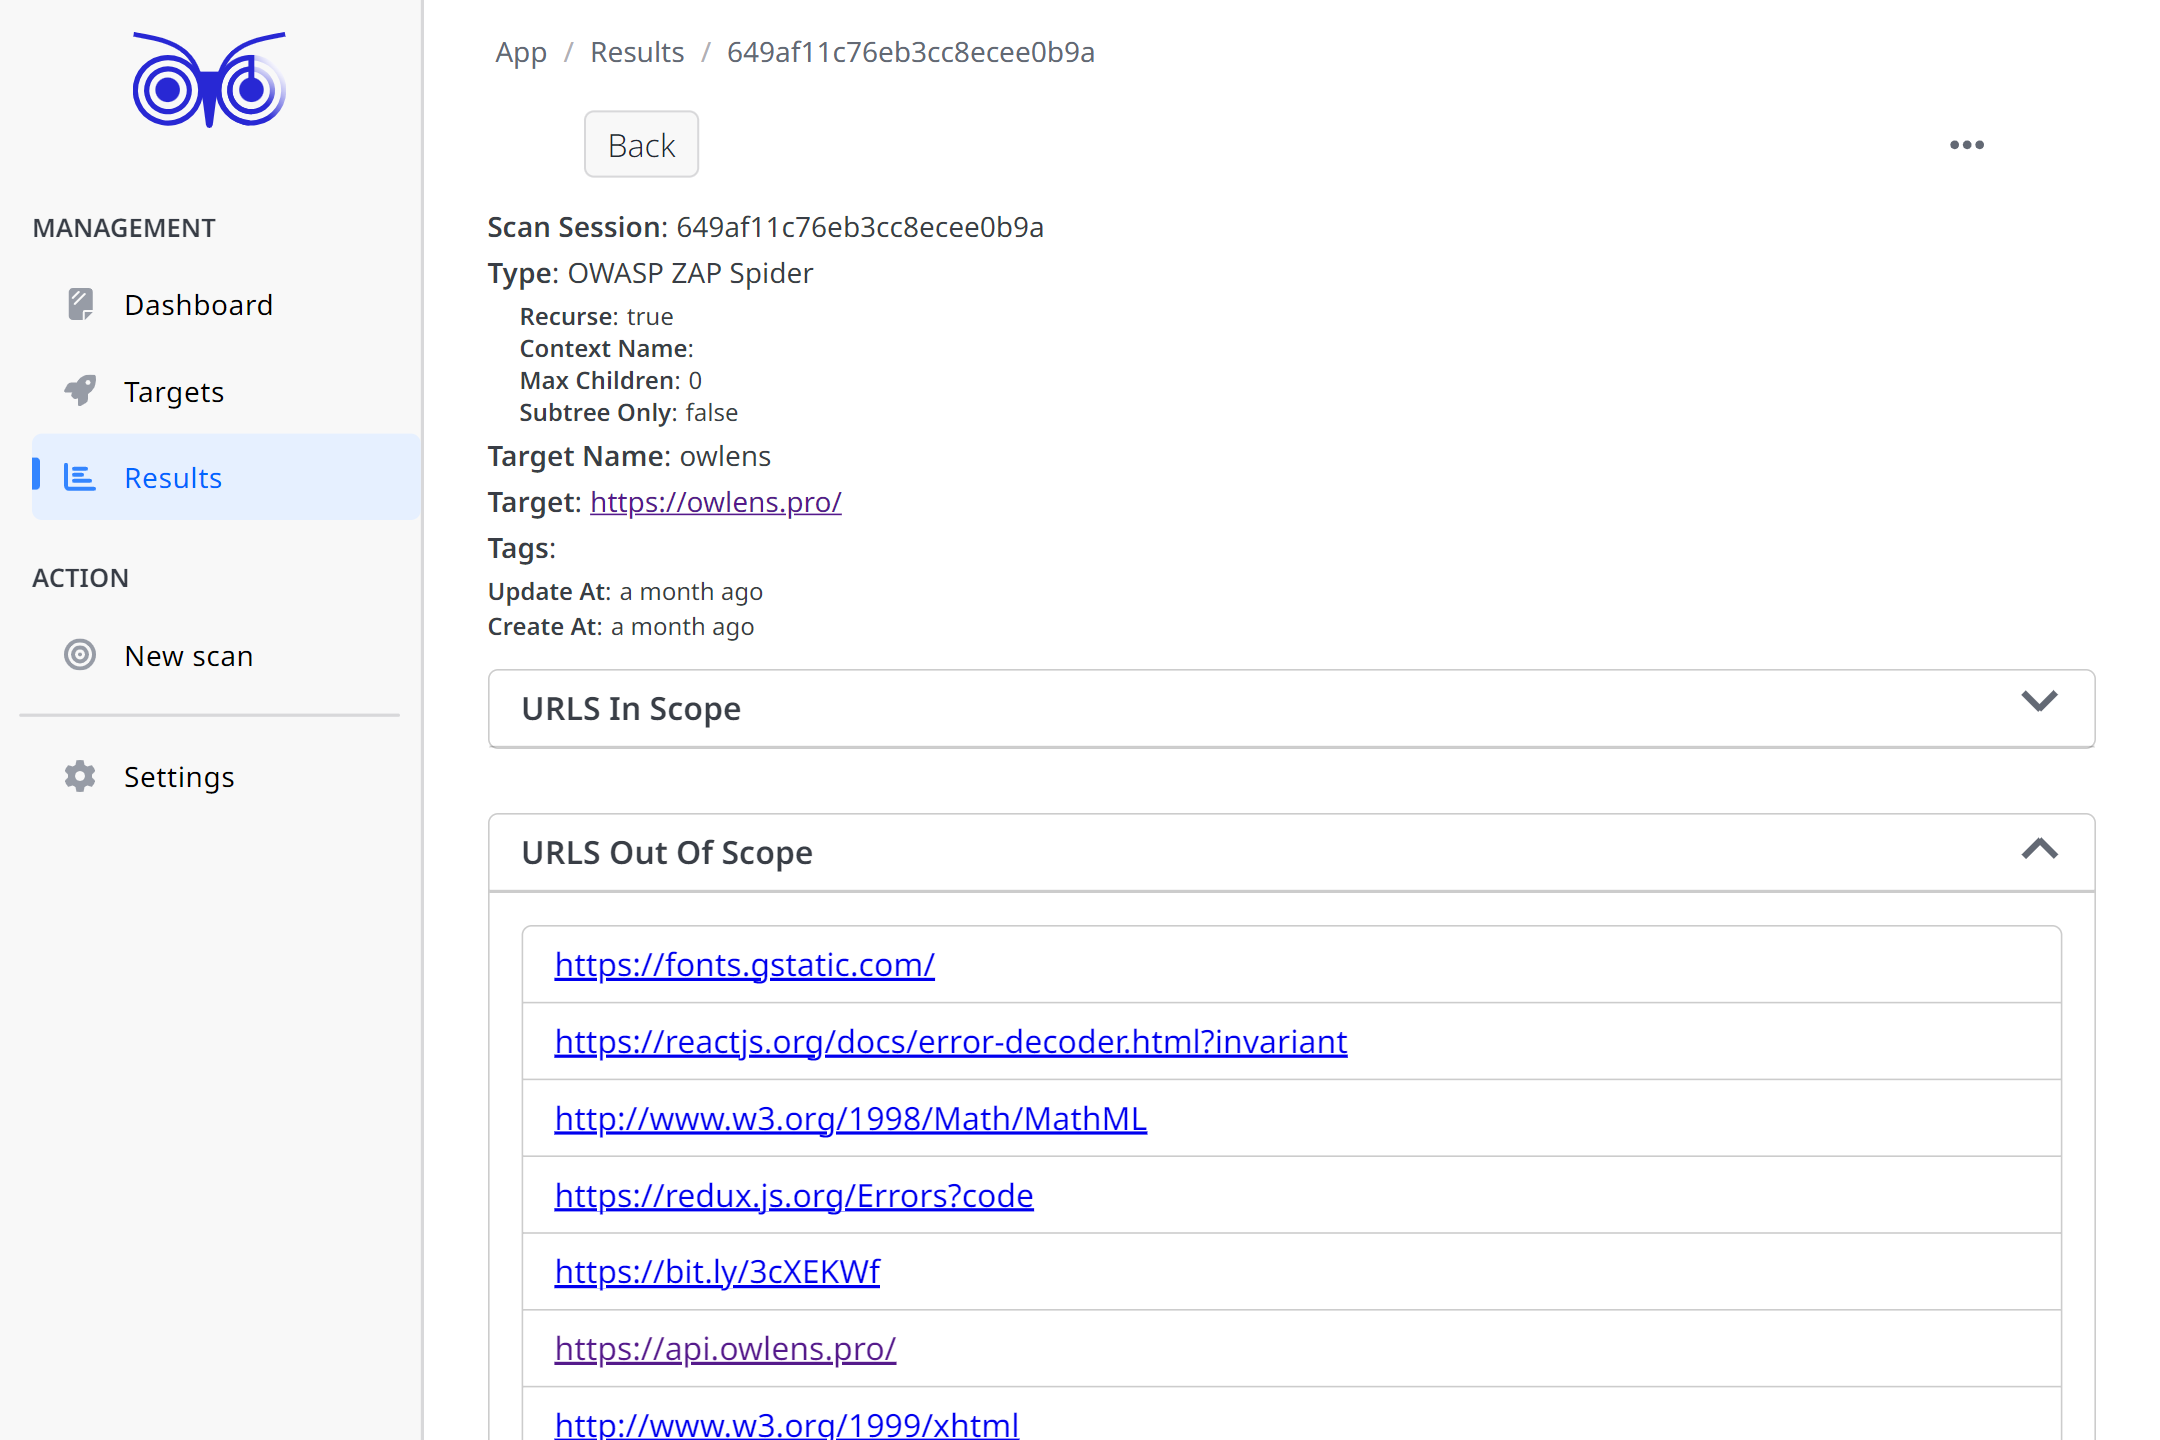
\includegraphics[width=\textwidth]{applied-thesis-chapters/chapter-6/Màn hình kết quả quét chi tiết Spider và bảng URLs Out Of Scope.png}
      \caption{Màn hình kết quả quét chi tiết Spider và bảng URLs Out Of Scope}
      \label{fig:ManHinhKetQuaQuetChiTietSpiderVaURLsOutOfScope}
\end{figure}

Các hình \textit{\ref{fig:ManHinhKetQuaQuetChiTietAjaxVaURLsInScope} \nameref{fig:ManHinhKetQuaQuetChiTietAjaxVaURLsInScope}} 
và \textit{\ref{fig:ManHinhKetQuaQuetChiTietAjaxVaURLsOutOfScope} \nameref{fig:ManHinhKetQuaQuetChiTietAjaxVaURLsOutOfScope}} 
thể hiện giao diện màn hình kết quả quét chi tiết của phiên quét loại Ajax.

\begin{figure}[H]
      \centering
      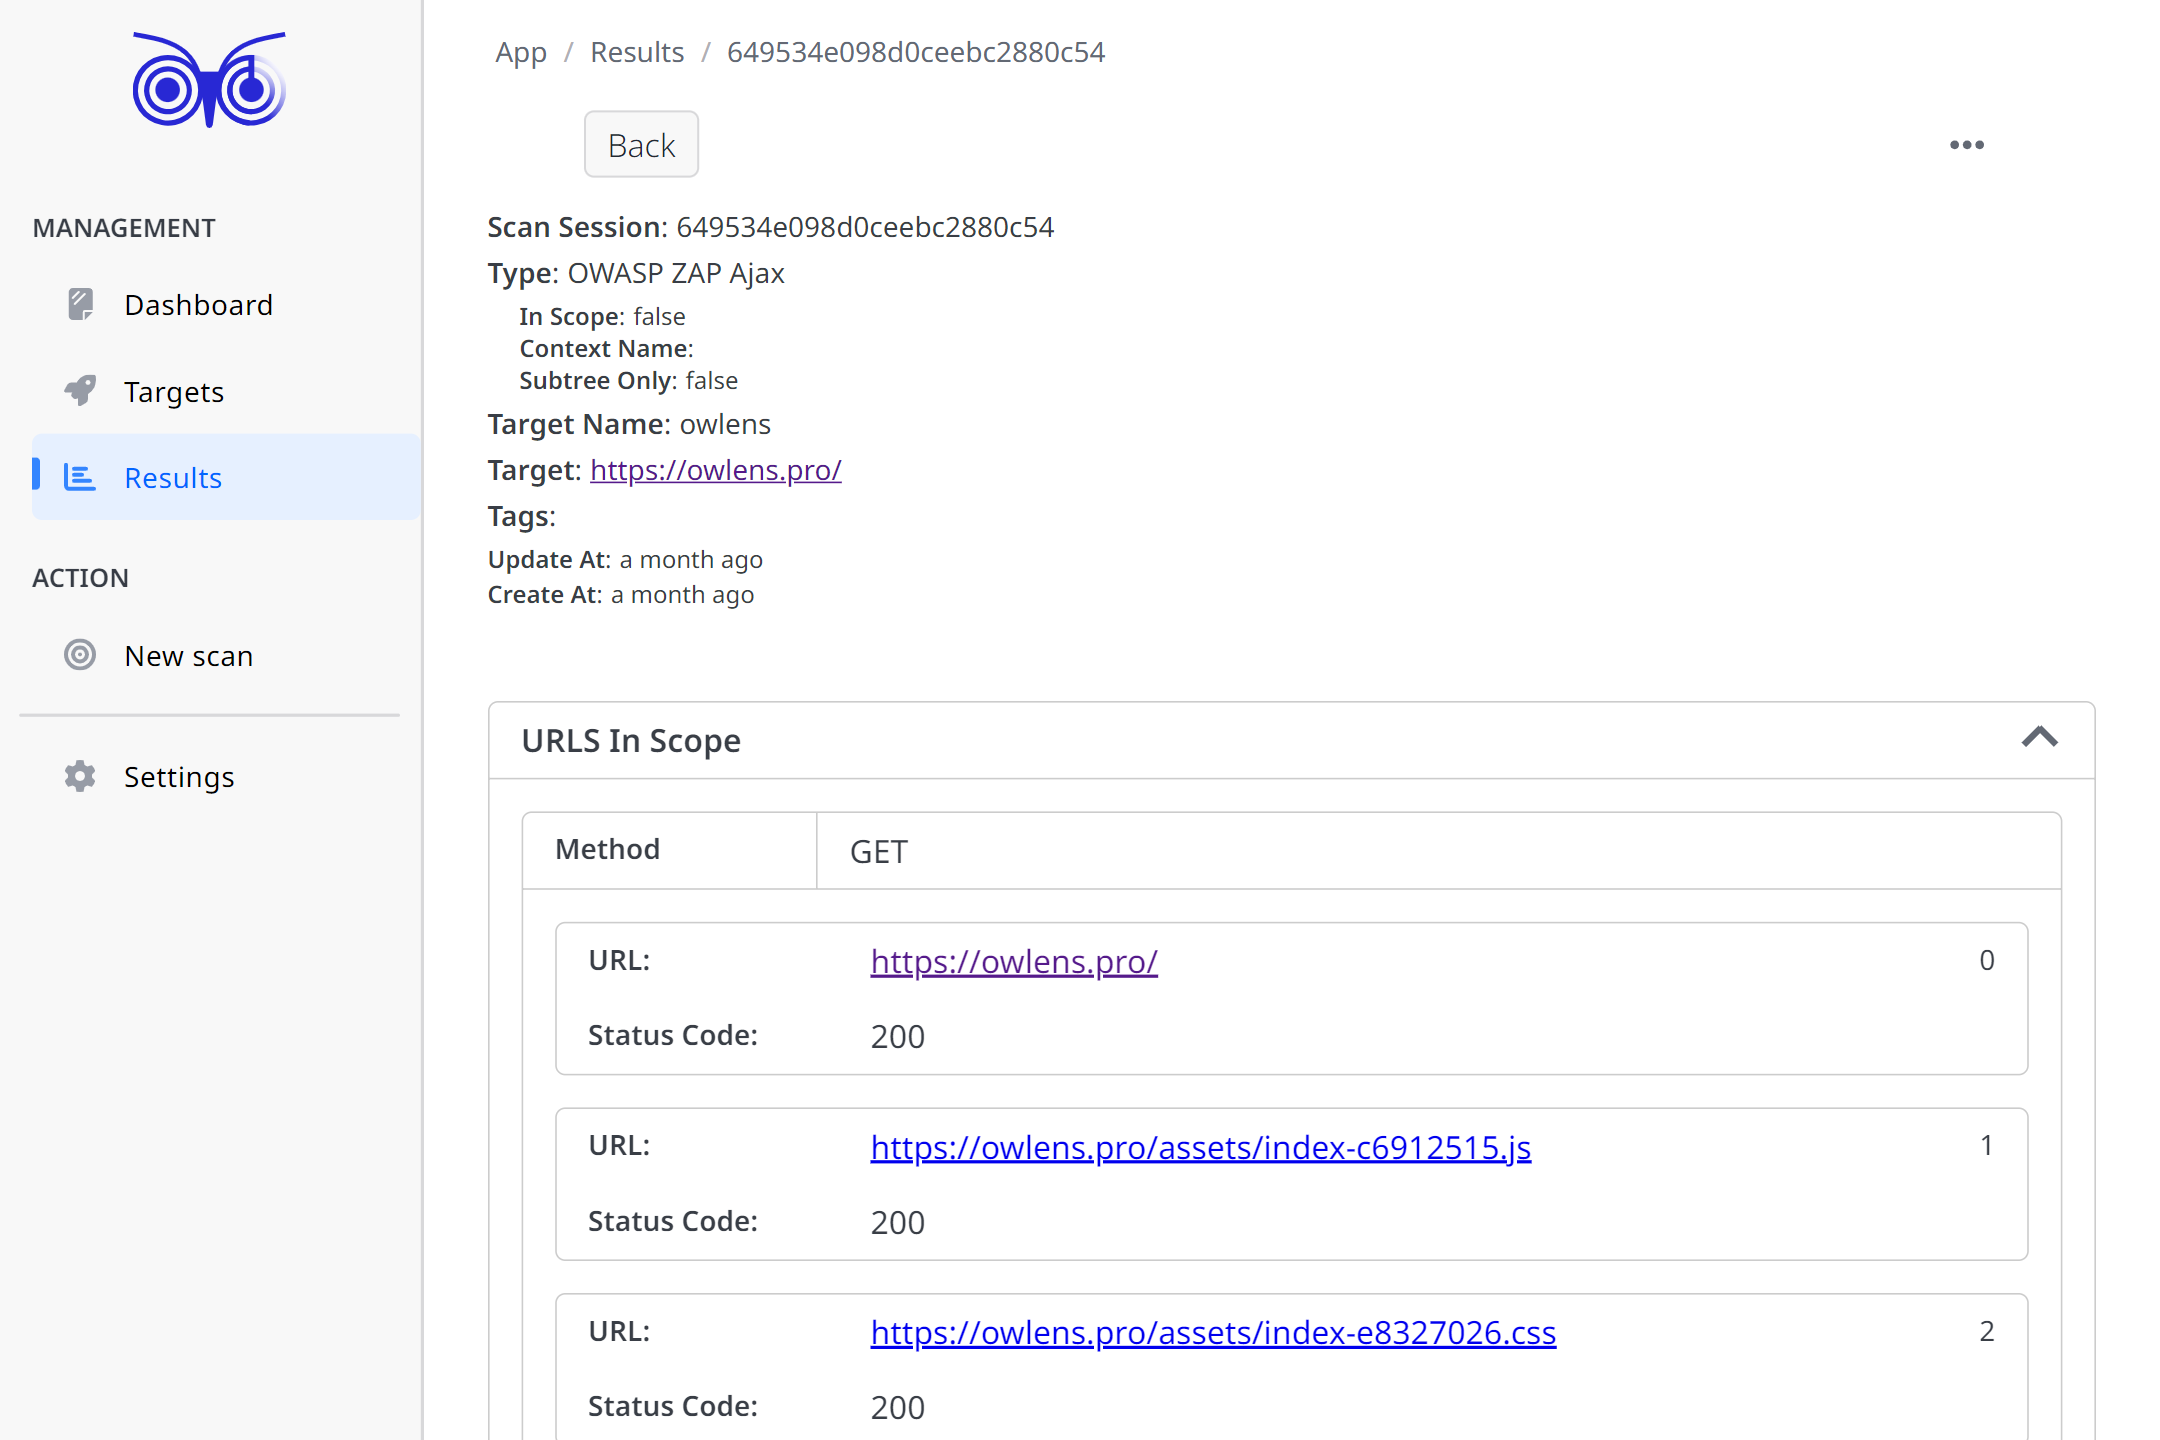
\includegraphics[width=\textwidth]{applied-thesis-chapters/chapter-6/Màn hình kết quả quét chi tiết Ajax và bảng URLs In Scope.png}
      \caption{Màn hình kết quả quét chi tiết Ajax và bảng URLs In Scope}
      \label{fig:ManHinhKetQuaQuetChiTietAjaxVaURLsInScope}
\end{figure}

\begin{figure}[H]
      \centering
      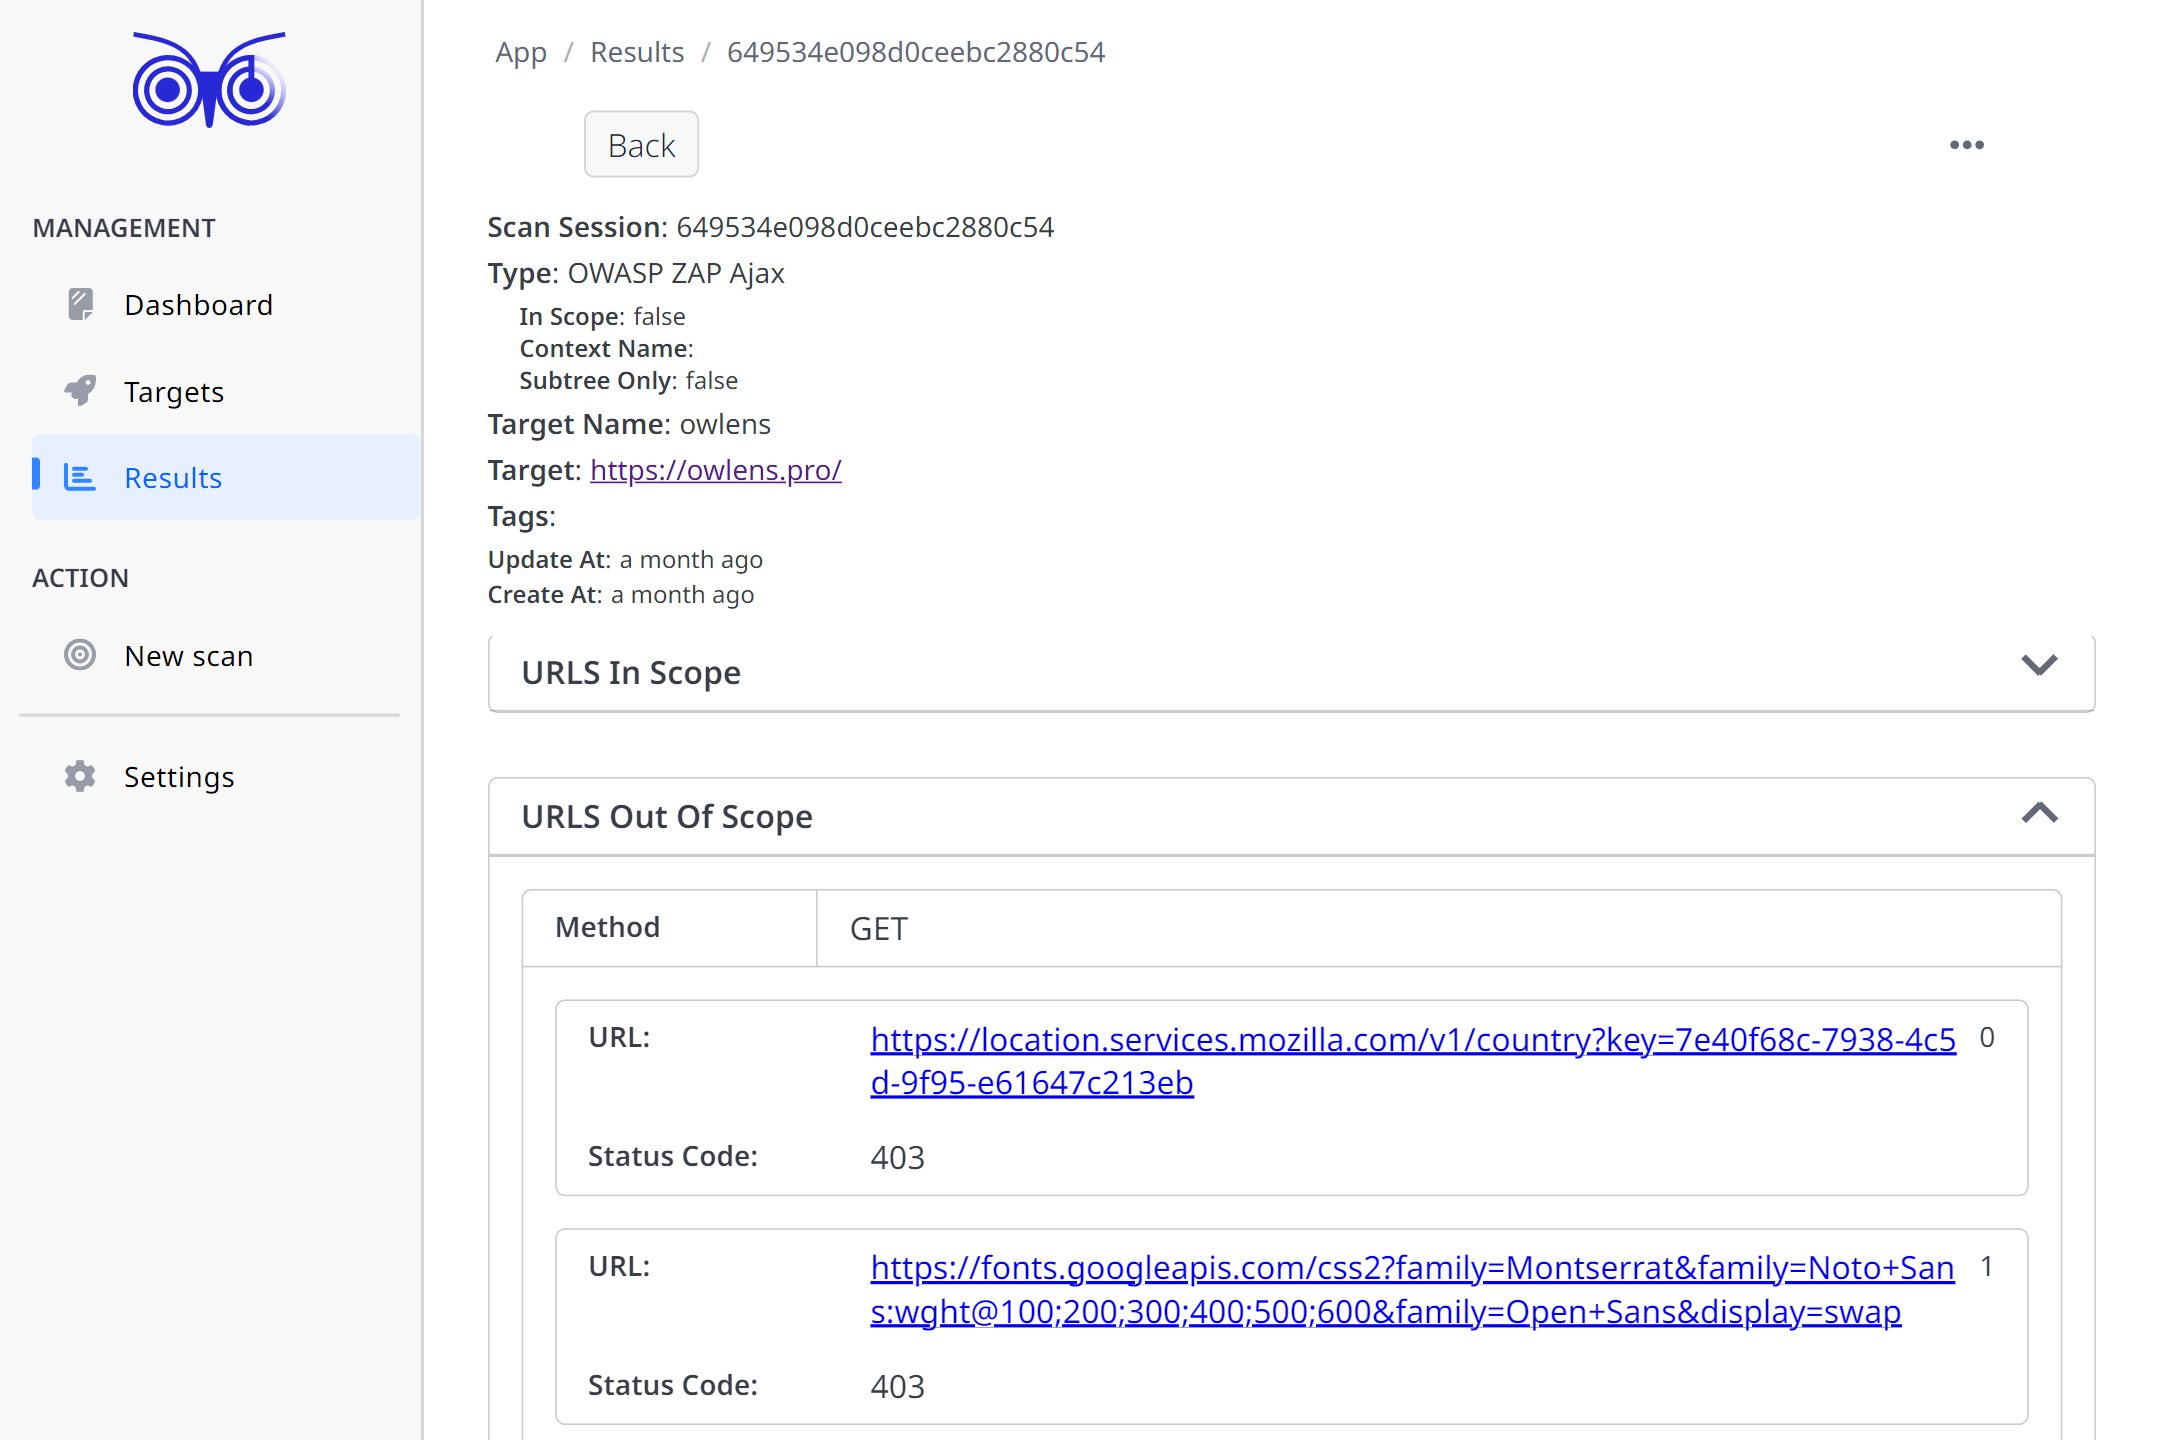
\includegraphics[width=\textwidth]{applied-thesis-chapters/chapter-6/Màn hình kết quả quét chi tiết Ajax và bảng URLs Out Of Scope.png}
      \caption{Màn hình kết quả quét chi tiết Ajax và bảng URLs Out Of Scope}
      \label{fig:ManHinhKetQuaQuetChiTietAjaxVaURLsOutOfScope}
\end{figure}

Các hình \textit{\ref{fig:ManHinhKetQuaQuetChiTietActiveVaAlertsSummary} \nameref{fig:ManHinhKetQuaQuetChiTietActiveVaAlertsSummary}}
, \textit{\ref{fig:ManHinhKetQuaQuetChiTietActiveVaAlertsInformation} \nameref{fig:ManHinhKetQuaQuetChiTietActiveVaAlertsInformation}} 
và \textit{\ref{fig:ManHinhKetQuaQuetChiTietActiveVaAlertsDetail} \nameref{fig:ManHinhKetQuaQuetChiTietActiveVaAlertsDetail}} 
thể hiện giao diện màn hình kết quả quét chi tiết của phiên quét loại Active.
Tương tự như Active, hình \textit{\ref{fig:ManHinhKetQuaQuetChiTietPassive} \nameref{fig:ManHinhKetQuaQuetChiTietPassive}} 
thể hiện cho phiên quét loại Passive.

\begin{figure}[H]
      \centering
      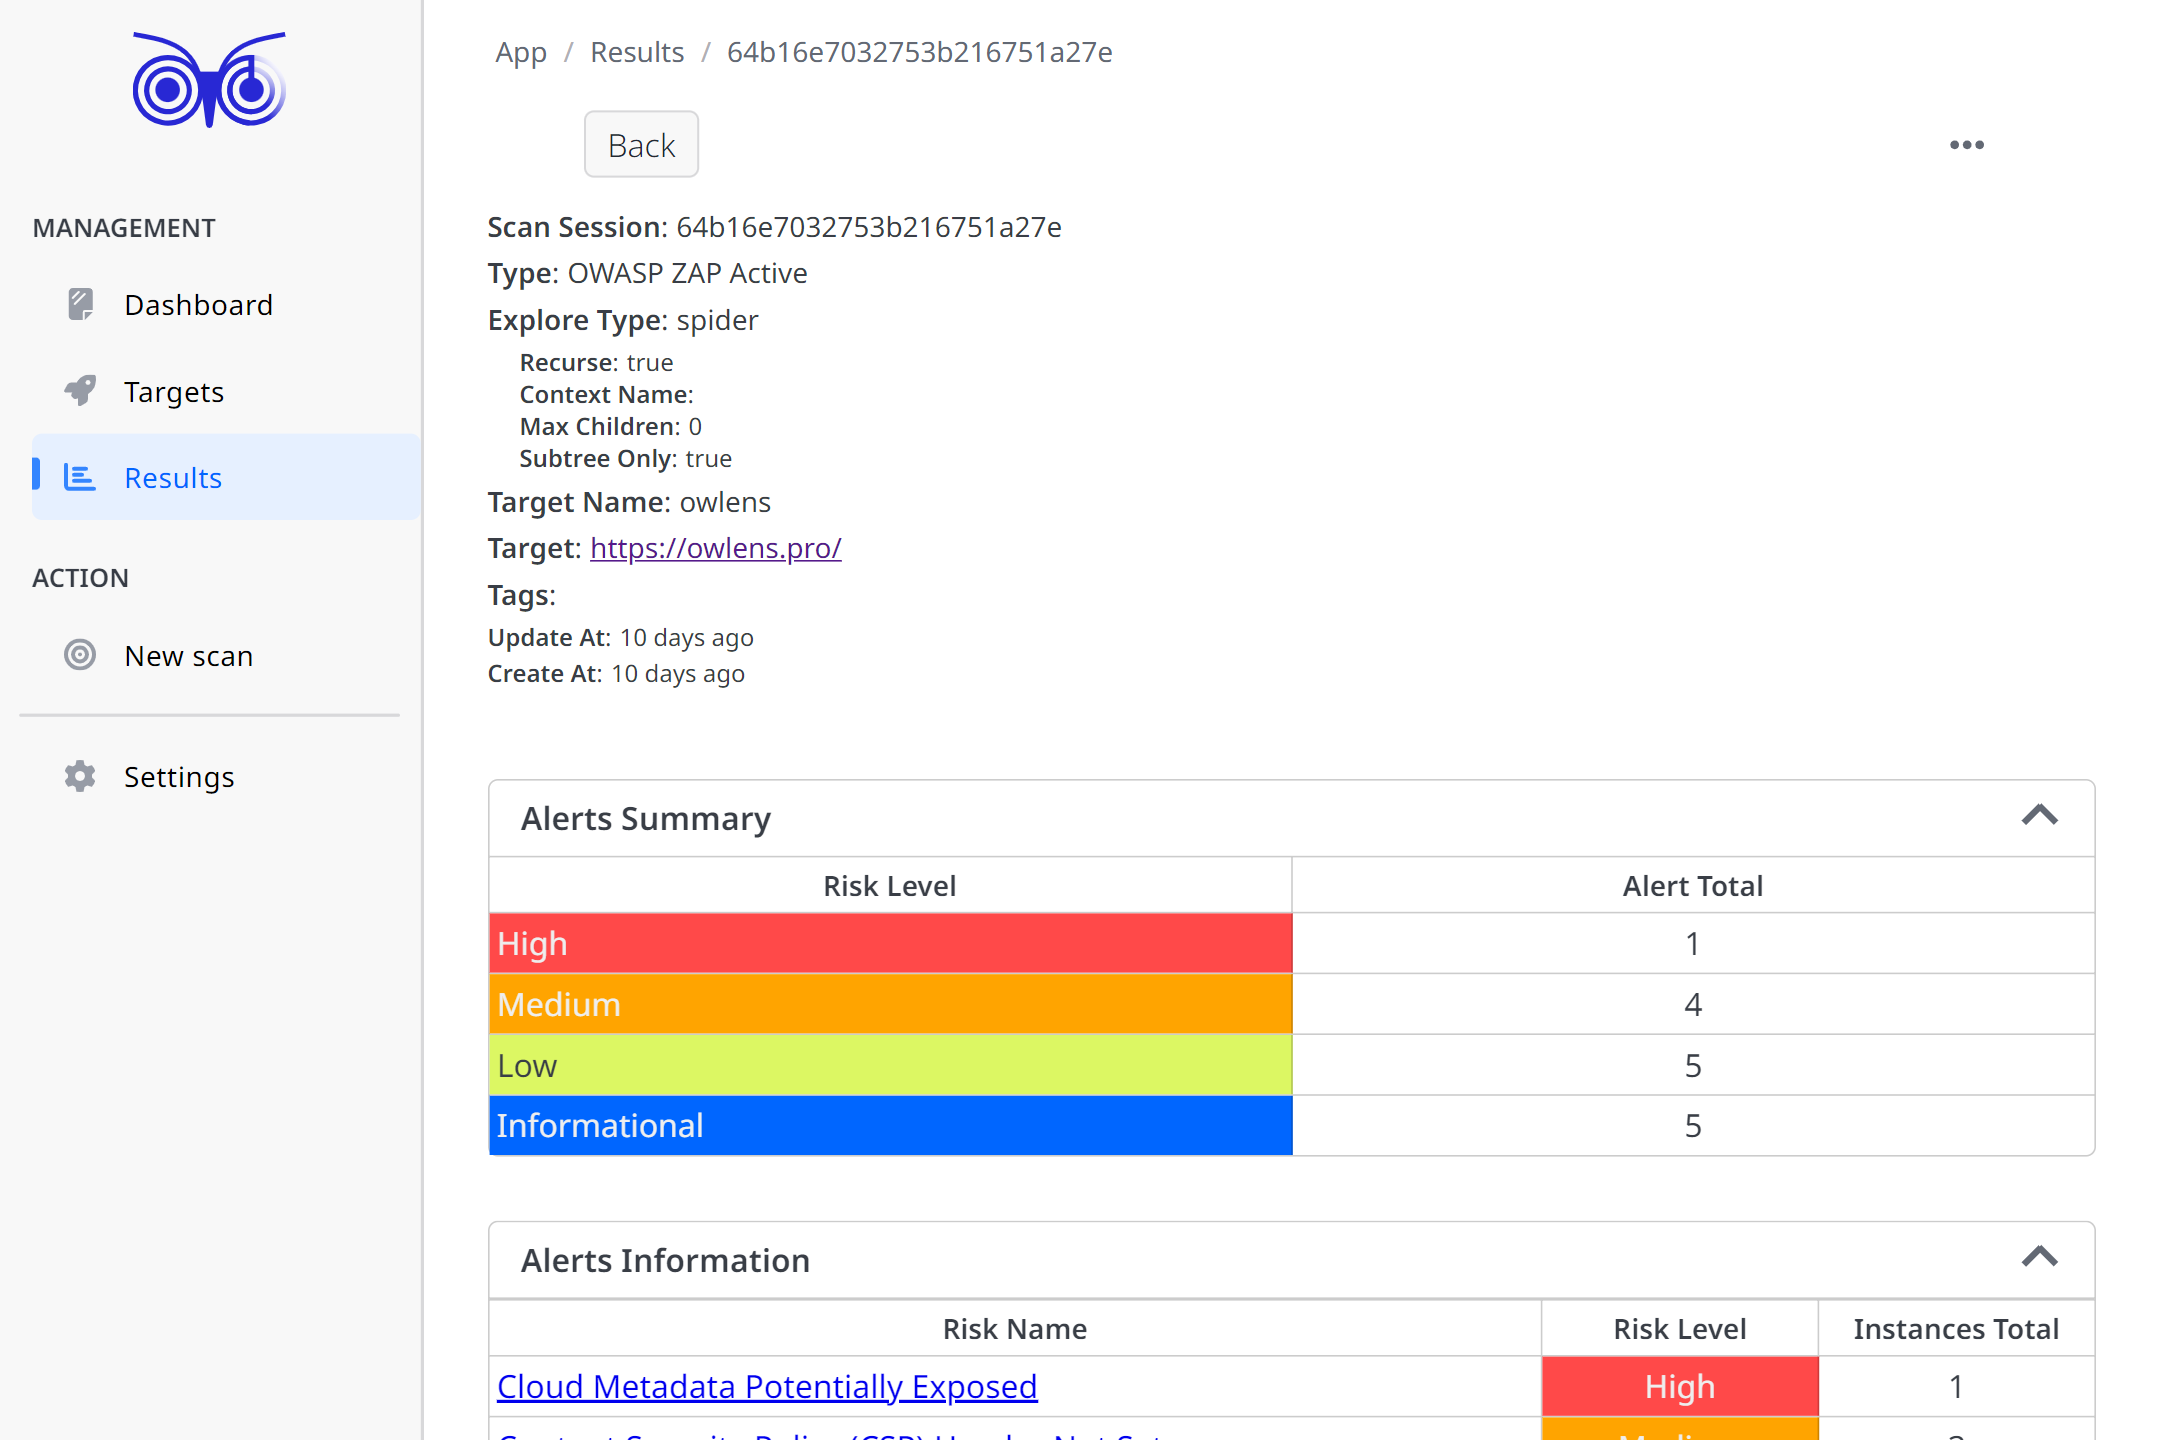
\includegraphics[width=\textwidth]{applied-thesis-chapters/chapter-6/Màn hình kết quả quét chi tiết Active và bảng Alerts Summary.png}
      \caption{Màn hình kết quả quét chi tiết Active và bảng Alerts Summary}
      \label{fig:ManHinhKetQuaQuetChiTietActiveVaAlertsSummary}
\end{figure}

\begin{figure}[H]
      \centering
      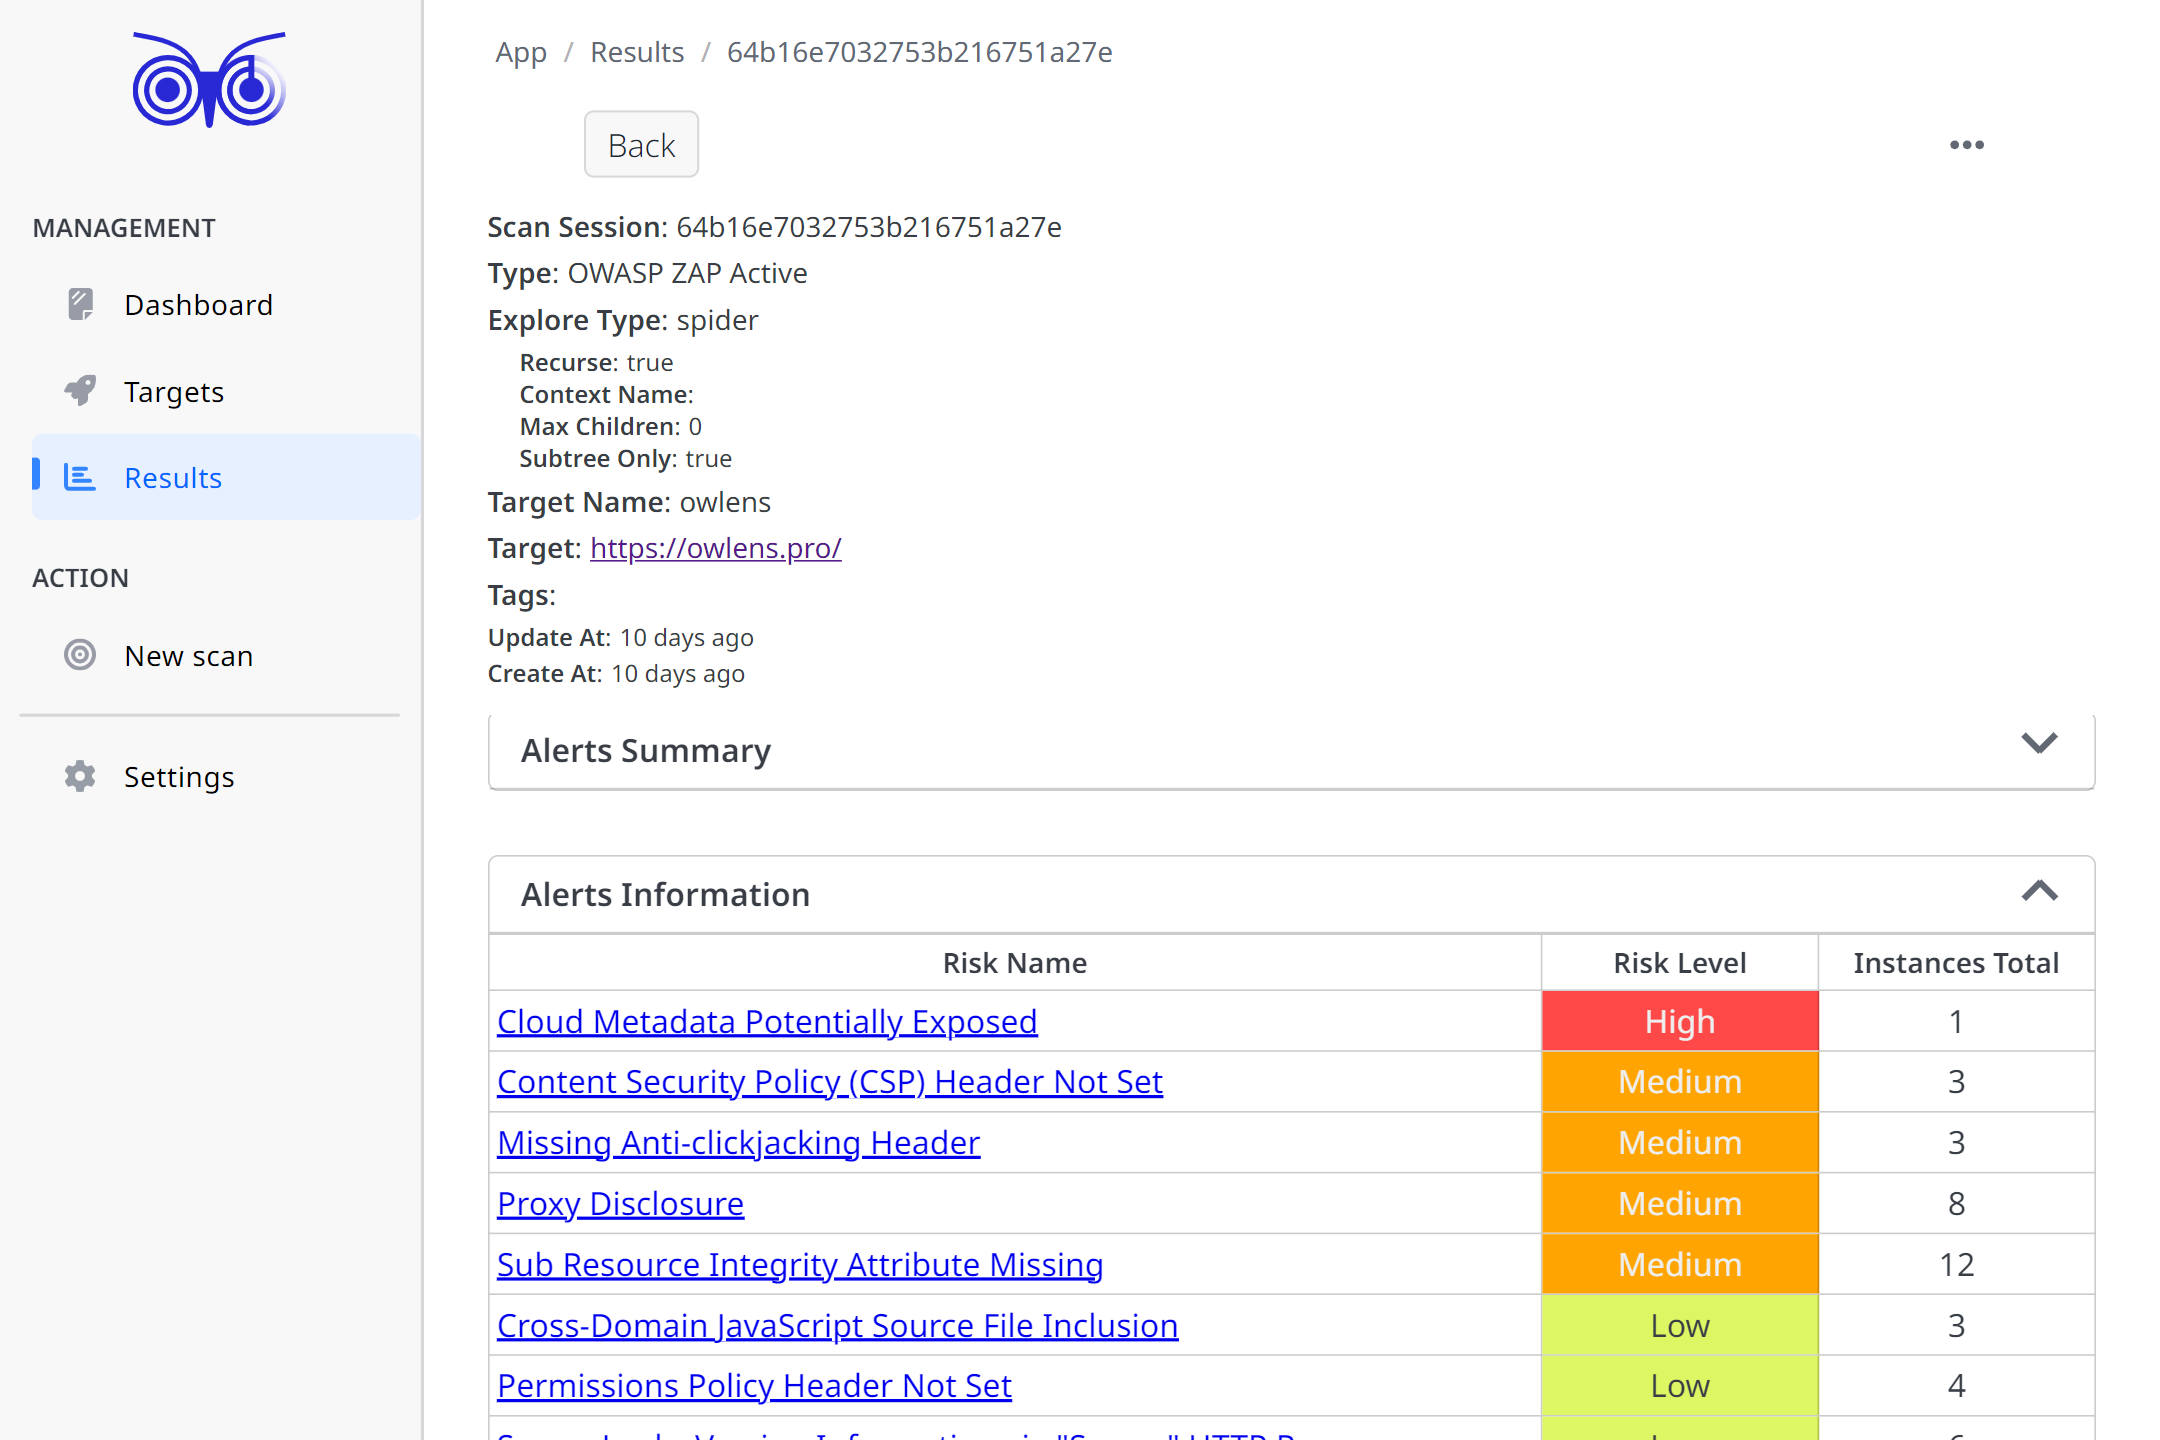
\includegraphics[width=\textwidth]{applied-thesis-chapters/chapter-6/Màn hình kết quả quét chi tiết Active và bảng Alerts Information.png}
      \caption{Màn hình kết quả quét chi tiết Active và bảng Alerts Information}
      \label{fig:ManHinhKetQuaQuetChiTietActiveVaAlertsInformation}
\end{figure}

\begin{figure}[H]
      \centering
      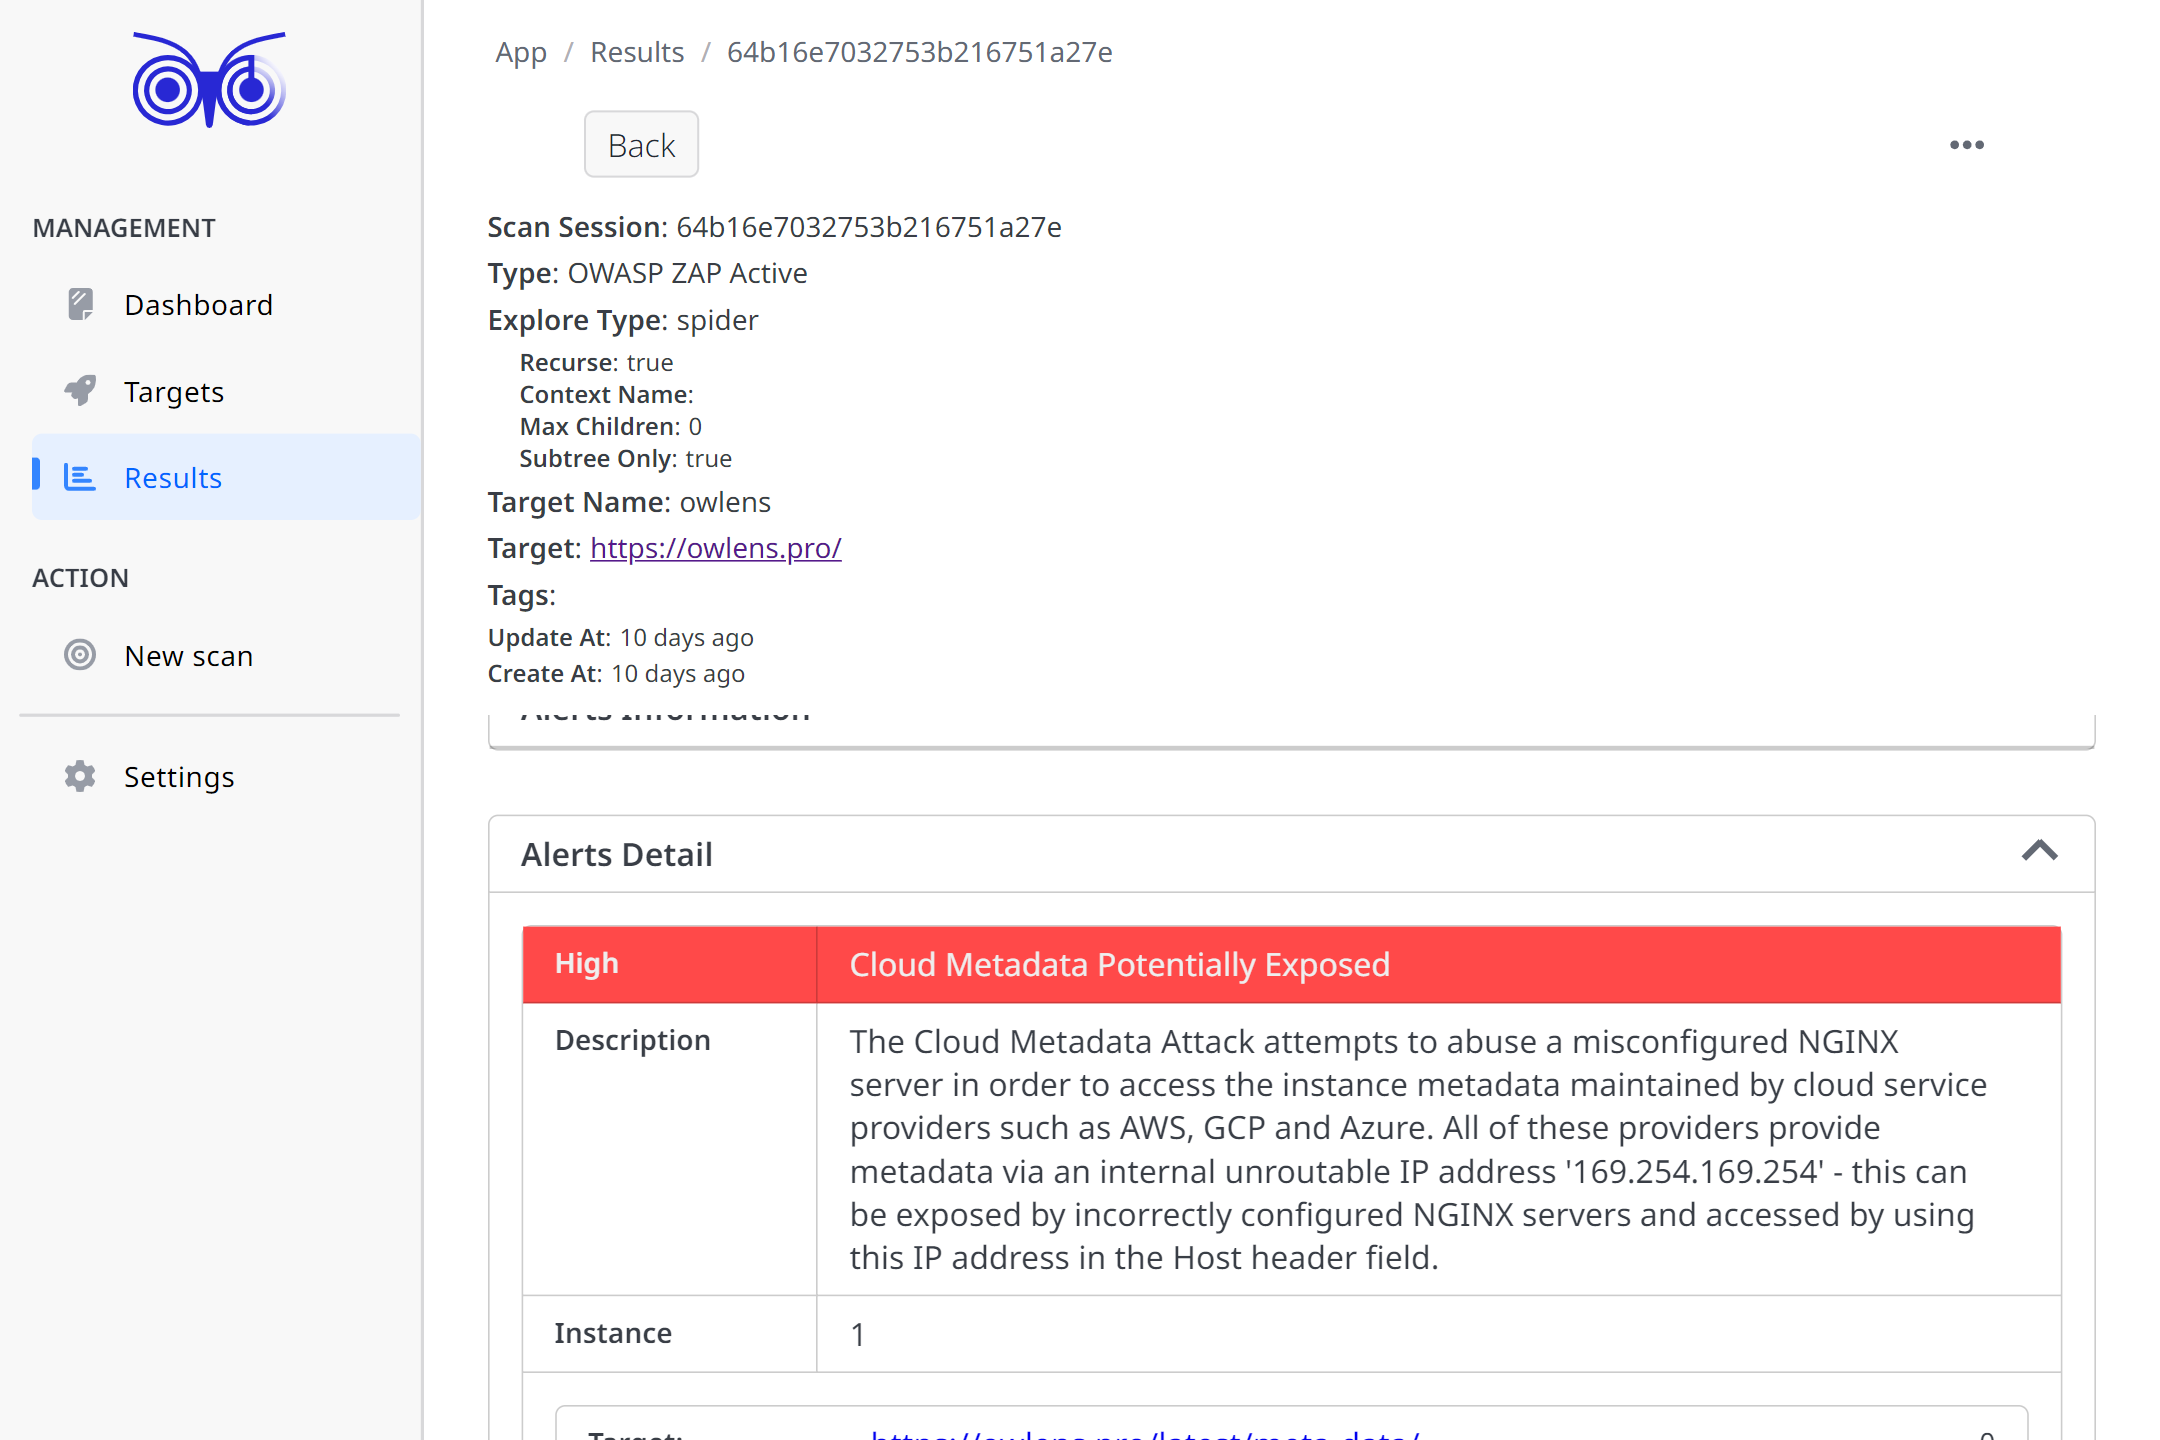
\includegraphics[width=\textwidth]{applied-thesis-chapters/chapter-6/Màn hình kết quả quét chi tiết Active và bảng Alerts Detail.png}
      \caption{Màn hình kết quả quét chi tiết Active và bảng Alerts Detail}
      \label{fig:ManHinhKetQuaQuetChiTietActiveVaAlertsDetail}
\end{figure}

\begin{figure}[H]
      \centering
      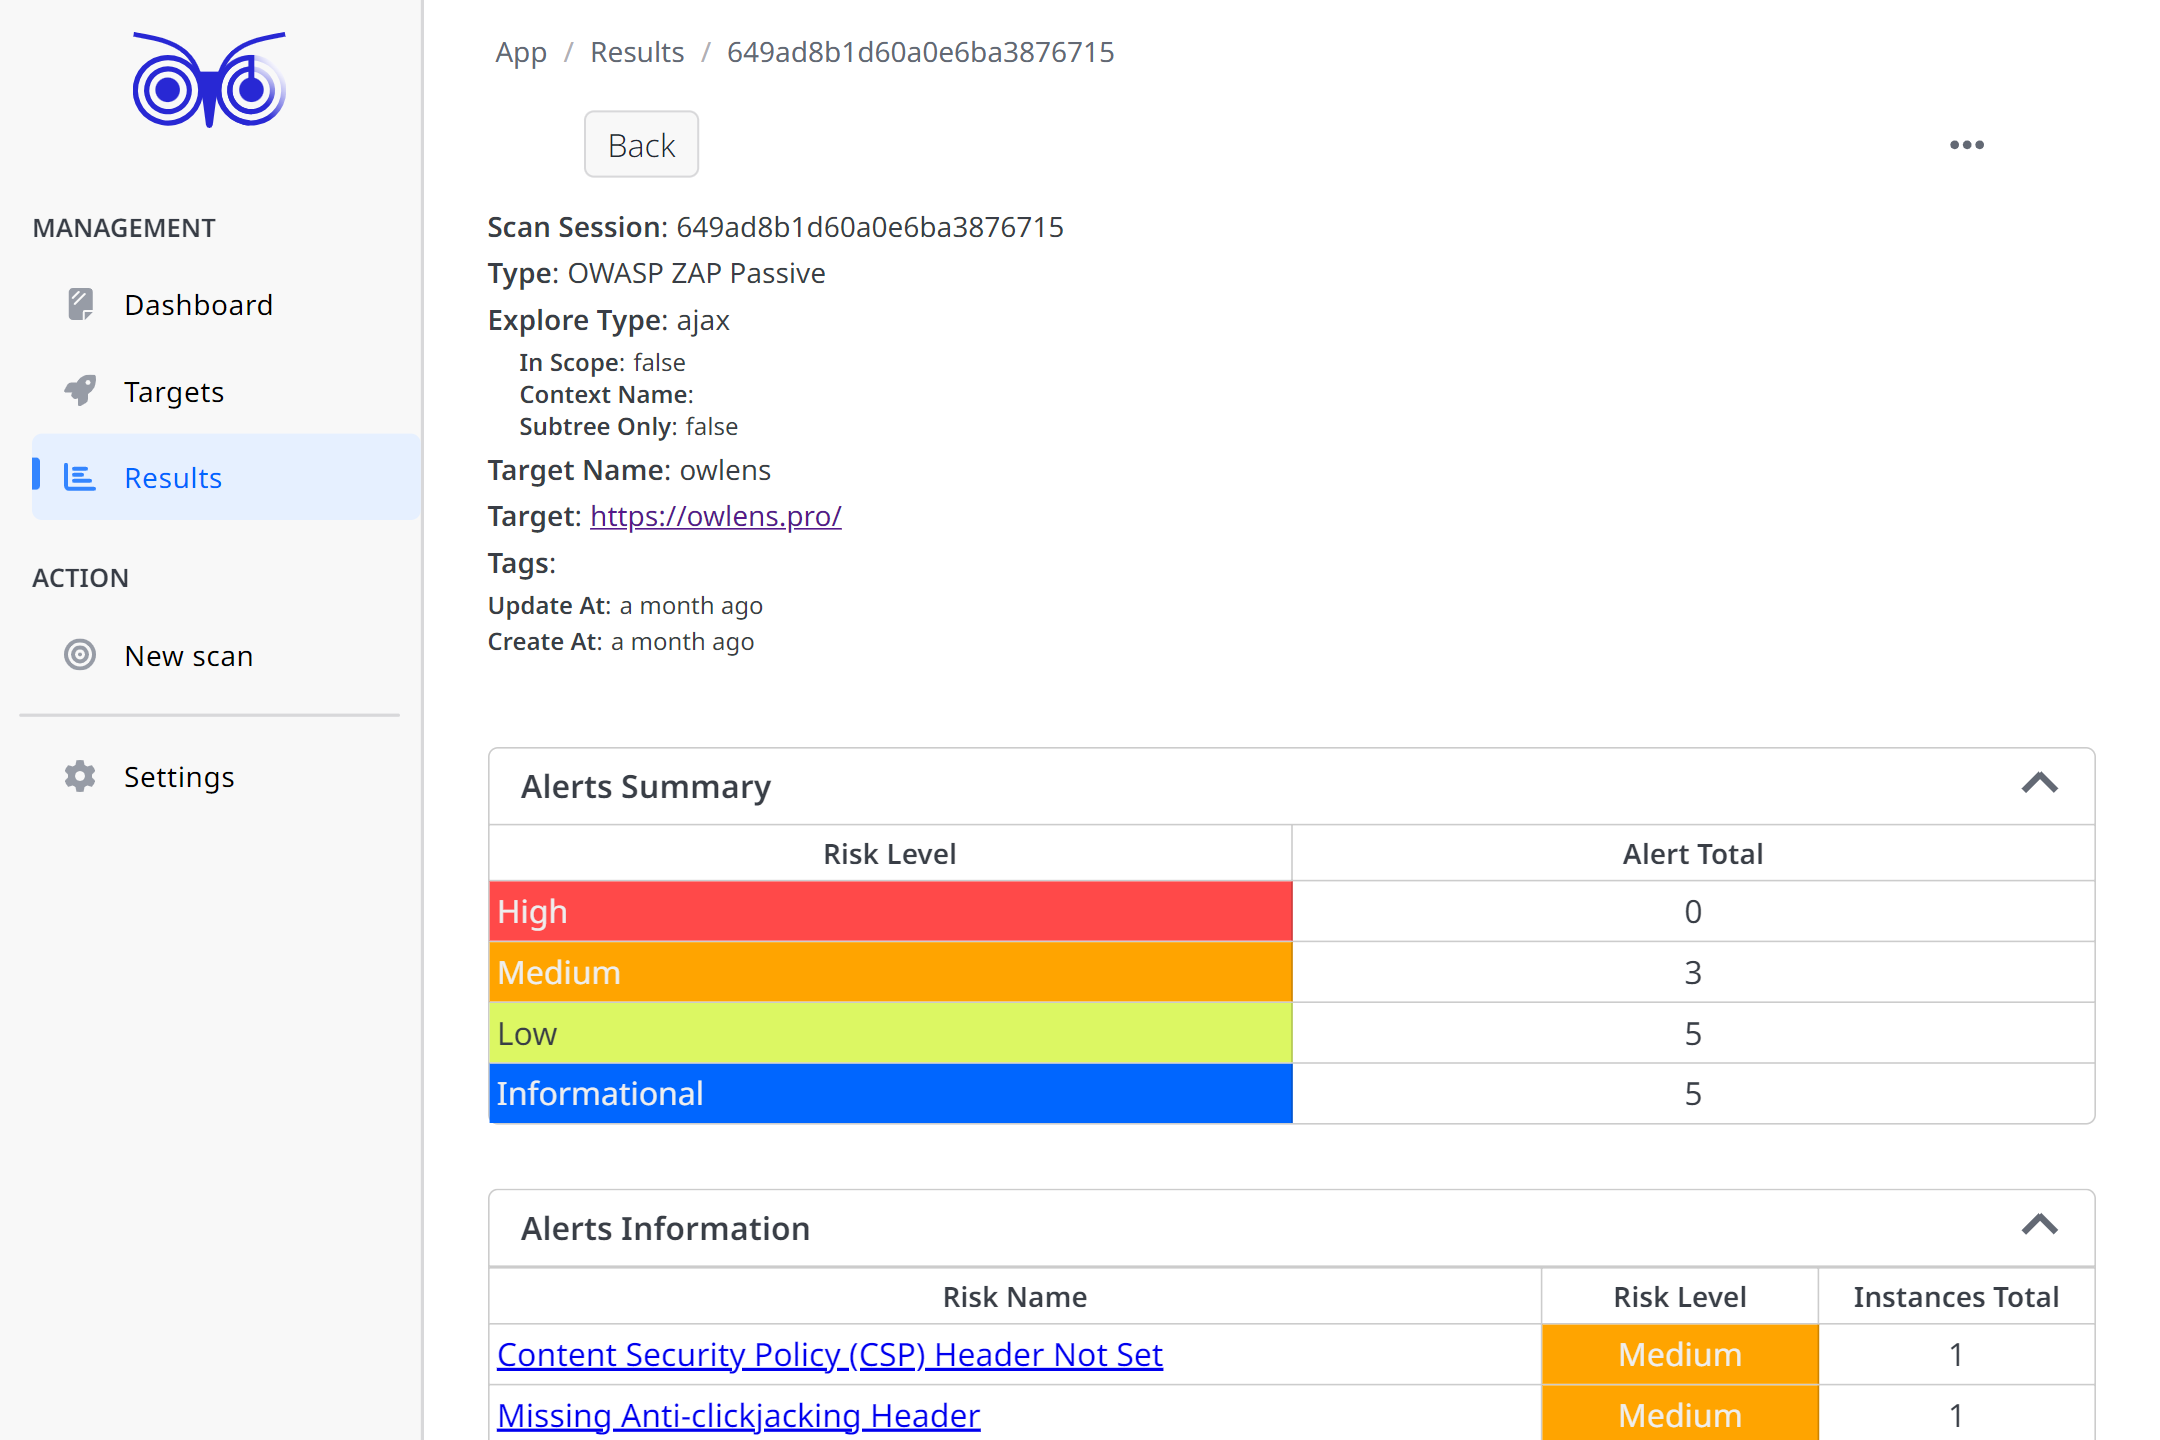
\includegraphics[width=\textwidth]{applied-thesis-chapters/chapter-6/Màn hình kết quả quét chi tiết Passive.png}
      \caption{Màn hình kết quả quét chi tiết Passive}
      \label{fig:ManHinhKetQuaQuetChiTietPassive}
\end{figure}

Như đã trình bày ở mục x....., ở màn hình này, đối với Passive và Active sẽ giống nhau ở "as12ec21ewfefwe" và chỉ khác nhau ở "thông tin session(coi lại để sửa cho nhất quán)"
